\chapter{Differential Equations and Analysis}
\label{chap:diffeq_complex}
\markboth{Differential Equations and Analysis}{Differential Equations and Analysis}

\begin{remark}[Positioning of this chapter]\label{rem:diffeq_chapter_positioning}
This chapter systematically applies the analytic tools established in the `Functions and Limits' chapter and the series/convolution framework established in the `Series and Convolution' chapter to four classes of analysis object: \textbf{differential equations} (integral curves of direction fields), \textbf{complex analysis} (analytic functions on the complex plane), \textbf{complex analyticity} (holomorphy, power-series expansions, residues) and \textbf{quaternion analysis and analyticity} (the exponential map and rotation representations in a non-commutative space). The core themes are: a differential equation is the integral curve of a direction field; an integral equation is a convolution equation of a trend kernel; conservation laws and first integrals are the constraints on the existence of periodic orbits; Floquet theory is the direct realisation of translation periodicity in differential equations; complex analysis and complex analyticity rebuild the direction--trend duality on the complex plane; and quaternionic analyticity lifts this duality to a non-commutative algebra, realising three-dimensional rotations through the exponential map and conjugation.

This chapter finally introduces the three fundamental differential operators---gradient, divergence and curl---and establishes the algebraic identities between them; the assumptions, ranges of applicability and boundary conditions for the three are given uniformly in the `Vector Analysis' chapter (\cref{sec:trans_scale_rotate}).

\textbf{On power series and Laurent series}: the general theory of series---Taylor series, Laurent series, the Cauchy--Hadamard radius-of-convergence formula and so on---has already been established systematically in Chapter~\ref{chap:series_conv}, `Series and Convolution' (\cref{def:taylor_series,def:laurent_series,thm:cauchy_hadamard,thm:laurent_expansion}). This chapter does not repeat that general theory; it uses its conclusions only in the context of complex analysis, and focuses on what is peculiar to complex analysis---the local expansion of analytic functions, the isolation of zeros, the classification of isolated singularities and the residue theorem.

\textbf{Guide to the seven themes of this chapter}: Translation---differential equations with periodic coefficients and Floquet theory (\S\ref{sec:floquet}), the $2\pi i$-periodicity of the complex exponential function (Proposition \ref{prop:complex_exp_periodicity}); Scaling---dissipative systems and volume contraction (\S\ref{sec:three_operators}), the stretch of the modulus of a complex number; Rotation---Hamiltonian systems and circulation (\S\ref{sec:three_operators}), the rotational period of a complex function, the conjugation action of quaternion rotations (\S\ref{sec:quaternion_analysis}); Conservation---first integrals (\S\ref{sec:first_integrals}), the Noether-type correspondence (Proposition \ref{prop:noether_ode}), Liouville's formula (Proposition \ref{prop:liouville_formula}), the rigidity of complex analyticity (\S\ref{sec:complex_analysis}); Symmetry---the classification of the three operator systems (Theorem \ref{thm:three_operator_periodic}), complex conjugation symmetry, quaternion conjugation symmetry; Closure---limit cycles and the Poincaré--Bendixson theorem (\S\ref{sec:ode_phase}), the closed contour of Cauchy's integral theorem (\S\ref{sec:cauchy_theory}); Period---Floquet multipliers (\S\ref{sec:floquet}), the imaginary period of the complex exponential, the $2\pi$-periodicity of the quaternion exponential.
\end{remark}

\begin{figure}[htbp]
\centering
\begin{tikzpicture}[
  font=\small,
  obj/.style={draw, rounded corners, fill=blue!8, minimum width=2.5cm, minimum height=0.8cm, align=center},
  theme/.style={draw, rounded corners, fill=green!10, minimum width=1.4cm, minimum height=0.6cm, align=center, font=\footnotesize},
  arr/.style={->, thick, >=stealth}
]
  \node[obj] (ode) {Differential equations\\integral curves of direction fields};
  \node[obj, right=1.0cm of ode] (ca) {Complex analysis\\direction--trend duality};
  \node[obj, right=1.0cm of ca] (res) {Complex analyticity\\expansions and residues};
  \node[obj, right=1.0cm of res] (quat) {Quaternions\\non-commutative rotations};
  \node[theme, below=1.2cm of ode] (p) {Translation};
  \node[theme, right=0.3cm of p] (s) {Scaling};
  \node[theme, right=0.3cm of s] (r) {Rotation};
  \node[theme, right=0.3cm of r] (c) {Conservation};
  \node[theme, right=0.3cm of c] (sym) {Symmetry};
  \node[theme, right=0.3cm of sym] (cl) {Closure};
  \node[theme, right=0.3cm of cl] (per) {Period};
  \node[draw, dashed, rounded corners, fit=(p)(per), inner sep=6pt] (themes) {};
  \node[below=0.1cm of themes, font=\footnotesize] {The seven themes run through the four classes of object};
  \foreach \x in {ode,ca,res,quat} {
    \draw[arr] (\x.south) -- ++(0,-0.35);
  }
  \draw[arr] (themes.north) -- ++(0,0.35);
\end{tikzpicture}
\caption{Overview of the structure of this chapter: the correspondence between the four classes of analysis object and the seven themes.}
\label{fig:diffeq_chapter_overview}
\end{figure}

\section{Ordinary Differential Equations: Integral Curves of Direction Fields}\label{sec:ode_basic}

\subsection{Basic Definitions, Existence and Uniqueness}

\begin{definition}[Ordinary Differential Equation]\label{def:ode}
Let $y: \mathbb{R} \to \mathbb{R}^n$ be an unknown vector-valued function. An \textbf{$n$-dimensional first-order system of ordinary differential equations} is
\[
\frac{dy}{dt} = \mathbf{F}(t, y),
\]
where $\mathbf{F}: \mathbb{R} \times \mathbb{R}^n \to \mathbb{R}^n$ is a given vector field. If $\mathbf{F}$ does not depend explicitly on $t$, the equation is called \textbf{autonomous}. If $\mathbf{F}(t+T, y) = \mathbf{F}(t, y)$, it is called a \textbf{periodically driven system}.

\textbf{Definition of a solution}: a function $y: I \to \mathbb{R}^n$ (with $I$ an interval) is called a \textbf{solution} of the equation on $I$ if $y$ is differentiable on $I$ and $y'(t) = \mathbf{F}(t, y(t))$ for every $t \in I$.
\end{definition}

\begin{definition}[Initial-Value Problem]\label{def:ivp}
Given $(t_0, y_0) \in \mathbb{R} \times \mathbb{R}^n$, the \textbf{initial-value problem} (IVP) is
\[
\frac{dy}{dt} = \mathbf{F}(t, y), \qquad y(t_0) = y_0.
\]
$y_0$ is called the \textbf{initial value} or the \textbf{initial condition}.
\end{definition}

\begin{definition}[Lipschitz Condition]\label{def:lipschitz}
Let $\mathbf{F}: D \subseteq \mathbb{R} \times \mathbb{R}^n \to \mathbb{R}^n$. We say that $\mathbf{F}$ satisfies the \textbf{Lipschitz condition} in $y$ on $D$ (with Lipschitz constant $L > 0$) if for any $(t, y_1), (t, y_2) \in D$,
\[
\|\mathbf{F}(t, y_1) - \mathbf{F}(t, y_2)\| \le L\|y_1 - y_2\|.
\]
\end{definition}

\begin{figure}[htbp]
\centering
\begin{tikzpicture}[
  node distance=0.8cm and 1.0cm,
  box/.style={draw, rounded corners, fill=orange!10, align=center, inner sep=5pt, font=\small},
  arr/.style={->, thick, >=stealth}
]
  \node[box] (ivp) {Initial-value problem\\$\dot y=\mathbf F(t,y),\;y(t_0)=y_0$};
  \node[box, right=of ivp] (int) {Equivalent integral equation\\$y=y_0+\int_{t_0}^t \mathbf F(s,y(s))ds$};
  \node[box, right=of int] (pic) {Picard iteration\\$y_{n+1}=y_0+\int \mathbf F(s,y_n)ds$};
  \node[box, below=of pic] (conv) {Uniform convergence\\$\sum \|y_{n+1}-y_n\|<\infty$};
  \node[box, left=of conv] (exist) {Existence and uniqueness of a solution\\Picard--Lindelöf};
  \node[box, left=of exist] (gron) {Gronwall's inequality\\controls the growth of perturbations};
  \draw[arr] (ivp) -- (int);
  \draw[arr] (int) -- (pic);
  \draw[arr] (pic) -- (conv);
  \draw[arr] (conv) -- (exist);
  \draw[arr] (exist) -- (gron);
\end{tikzpicture}
\caption{Road map of the Picard--Lindelöf proof of existence and uniqueness: the initial-value problem is converted into an integral equation, Picard iteration together with uniform convergence yields the solution, and Gronwall's inequality is finally used to prove uniqueness.}
\label{fig:picard_flow}
\end{figure}

\begin{lemma}[Gronwall's Inequality]\label{lem:gronwall}
Let $\varphi: [t_0, t_0+\alpha] \to [0, \infty)$ be continuous and satisfy
\[
\varphi(t) \le \varphi_0 + \int_{t_0}^t \beta \varphi(s)\,ds, \qquad t \in [t_0, t_0+\alpha],
\]
where $\varphi_0 \ge 0$ and $\beta \ge 0$ are constants. Then
\[
\varphi(t) \le \varphi_0\, e^{\beta(t-t_0)}, \qquad t \in [t_0, t_0+\alpha].
\]
Symmetrically, if $\varphi(t) \le \varphi_0 + \int_t^{t_0} \beta \varphi(s)\,ds$ ($t \le t_0$), then $\varphi(t) \le \varphi_0 e^{\beta(t_0-t)}$.
\end{lemma}

\begin{proof}
Define $\Phi(t) = \varphi_0 + \int_{t_0}^t \beta \varphi(s)\,ds$. Then $\Phi$ is continuously differentiable, $\Phi' = \beta \varphi \le \beta \Phi$, and $\Phi(t_0) = \varphi_0$. Let $\Psi(t) = \Phi(t) e^{-\beta(t-t_0)}$; then $\Psi'(t) = (\Phi'(t) - \beta\Phi(t)) e^{-\beta(t-t_0)} \le 0$, so $\Psi(t) \le \Psi(t_0) = \varphi_0$, that is, $\Phi(t) \le \varphi_0 e^{\beta(t-t_0)}$. Since $\varphi(t) \le \Phi(t)$, the claim follows. The left-hand case follows in the same way after the change of variable $t \mapsto -t$.
\end{proof}

\begin{theorem}[Picard--Lindelöf Existence and Uniqueness Theorem]\label{thm:picard_lindelof}
Let $\mathbf{F}(t, y)$ be continuous on the domain $D = \{(t, y) : |t-t_0| \le a, \|y - y_0\| \le b\}$ and satisfy the Lipschitz condition in $y$ (\cref{def:lipschitz}, with Lipschitz constant $L$). Then the initial-value problem $\frac{dy}{dt} = \mathbf{F}(t, y)$, $y(t_0) = y_0$ has a unique solution on the interval $|t-t_0| \le \alpha$, where $\alpha = \min(a, b/M)$ and $M = \max_{(t,y)\in D} \|\mathbf{F}(t,y)\|$.
\end{theorem}

\begin{proof}
\textbf{Step 1: reduction to an integral equation}. The initial-value problem is equivalent to the integral equation
\[
y(t) = y_0 + \int_{t_0}^t \mathbf{F}(s, y(s))\,ds.
\]
(If $y$ is a solution of the differential equation, integrating both sides gives the integral equation; if $y$ satisfies the integral equation, differentiating by the fundamental theorem of calculus gives the differential equation.)

\textbf{Step 2: Picard iteration}. Define the iteration sequence:
\[
y_0(t) = y_0, \qquad y_{n+1}(t) = y_0 + \int_{t_0}^t \mathbf{F}(s, y_n(s))\,ds.
\]
One must verify that $y_n(t)$ is defined on $|t-t_0| \le \alpha$ and that $\|y_n(t) - y_0\| \le b$. Use induction: for $n=0$ we have $\|y_0(t)-y_0\|=0\le b$, so the claim holds. Suppose that $\|y_n(t) - y_0\| \le b$; then
\[
\|y_{n+1}(t) - y_0\| \le \int_{t_0}^t \|\mathbf{F}(s, y_n(s))\|\,ds \le M |t - t_0| \le M\alpha \le b.
\]

\textbf{Step 3: proof that the iteration sequence converges}. Estimate $\|y_{n+1}(t) - y_n(t)\|$. By the Lipschitz condition,
\[
\|y_{n+1}(t) - y_n(t)\| \le \int_{t_0}^t L\|y_n(s) - y_{n-1}(s)\|\,ds.
\]
Prove by induction that
\[
\|y_{n+1}(t) - y_n(t)\| \le \frac{M L^n |t - t_0|^{n+1}}{(n+1)!}.
\]
Base step $n=0$: $\|y_1(t) - y_0\| \le M|t-t_0|$. Inductive step: assuming the claim for $n-1$, we get
\[
\|y_{n+1} - y_n\| \le \int_{t_0}^t L \cdot \frac{M L^{n-1} |s-t_0|^n}{n!}\,ds = \frac{M L^n |t-t_0|^{n+1}}{(n+1)!}.
\]
Hence the series $\sum_{n=0}^{\infty} \|y_{n+1} - y_n\|$ converges (by comparison with the exponential series), and the sequence of functions $\{y_n\}$ converges uniformly on $|t-t_0| \le \alpha$ to some continuous function $y$.

\textbf{Step 4: the limit is a solution}. Passing to the limit in the iteration formula (the integral and the limit may be interchanged, by uniform convergence) gives
\[
y(t) = y_0 + \int_{t_0}^t \mathbf{F}(s, y(s))\,ds.
\]

\textbf{Step 5: uniqueness}. Let $y_1, y_2$ be two solutions and put $\delta(t) = \|y_1(t) - y_2(t)\|$. By the Lipschitz condition,
\[
\delta(t) \le \int_{t_0}^t L\delta(s)\,ds \qquad (t \ge t_0).
\]
Applying Gronwall's inequality (Lemma \ref{lem:gronwall}) with $\varphi(t) = \delta(t)$, $\varphi_0 = 0$ and $\beta = L$ gives $\delta(t) \le 0$, that is, $\delta(t) = 0$. The case $t \le t_0$ is analogous. Hence $y_1 = y_2$.
\end{proof}

\begin{proposition}[Continuous Dependence of the Solution on the Initial Value]\label{prop:continuous_dependence}
Let $\mathbf{F}(t, y)$ satisfy the Lipschitz condition (with Lipschitz constant $L$). Then the solution $y(t; t_0, y_0)$ depends continuously on the initial value $y_0$:
\[
\|y(t; t_0, y_0) - y(t; t_0, \tilde{y}_0)\| \le e^{L|t-t_0|} \|y_0 - \tilde{y}_0\|.
\]
\end{proposition}

\begin{proof}
Let $y_1(t) = y(t; t_0, y_0)$, $y_2(t) = y(t; t_0, \tilde{y}_0)$ and $\delta(t) = \|y_1(t) - y_2(t)\|$. By the Lipschitz condition,
\[
\delta(t) \le \|y_0 - \tilde{y}_0\| + \int_{t_0}^t L\delta(s)\,ds \qquad (t \ge t_0).
\]
Applying Gronwall's inequality (Lemma \ref{lem:gronwall}) with $\varphi(t) = \delta(t)$, $\varphi_0 = \|y_0 - \tilde{y}_0\|$ and $\beta = L$, we obtain
\[
\delta(t) \le \|y_0 - \tilde{y}_0\|\, e^{L(t-t_0)}.
\]
The case $t \le t_0$ is given analogously by the left-hand Gronwall inequality: $\delta(t) \le \|y_0 - \tilde{y}_0\| e^{L(t_0-t)}$. Combining the two yields $\delta(t) \le \|y_0 - \tilde{y}_0\| e^{L|t-t_0|}$.
\end{proof}

\begin{property}[Differentiable Dependence of the Solution on Parameters]\label{prop:solution_smooth_dependence}
Let $\mathbf{F}(t, y, \mu)$ satisfy the Lipschitz condition in $(y, \mu)$, and let $\partial \mathbf{F}/\partial \mu$ be continuous. Then the solution $y(t; \mu)$ is differentiable with respect to the parameter $\mu$, and its variation $\partial y/\partial \mu$ satisfies the \textbf{variational equation}
\[
\frac{d}{dt}\frac{\partial y}{\partial \mu} = \frac{\partial \mathbf{F}}{\partial y}\frac{\partial y}{\partial \mu} + \frac{\partial \mathbf{F}}{\partial \mu}, \qquad \frac{\partial y}{\partial \mu}(t_0) = 0.
\]
\end{property}

\subsection{Linear Ordinary Differential Equations}

\begin{definition}[First-Order Linear Homogeneous System]\label{def:linear_homogeneous_ode}
A first-order linear homogeneous ordinary differential equation has the form $\frac{dy}{dt} = A(t) y$. Its solution can be written as $y(t) = \Phi(t, t_0) y_0$, where $\Phi(t, t_0)$ is the \textbf{state transition matrix}, satisfying $\frac{d}{dt}\Phi(t, t_0) = A(t)\Phi(t, t_0)$ and $\Phi(t_0, t_0) = I$. When $A$ is a constant matrix, $\Phi(t, 0) = e^{At}$.
\end{definition}

\begin{property}[Basic Properties of the State Transition Matrix]\label{prop:stm_properties}
The state transition matrix $\Phi(t, t_0)$ satisfies:
\begin{enumerate}[label=(\roman*)]
    \item \textbf{Invertibility}: $\Phi(t, t_0)$ is invertible for every $t$, and $\Phi^{-1}(t, t_0) = \Phi(t_0, t)$.
    \item \textbf{Chain property}: $\Phi(t_2, t_0) = \Phi(t_2, t_1)\Phi(t_1, t_0)$.
    \item \textbf{Exponential form}: if $A(t)$ commutes with $\int_{t_0}^t A(s)\,ds$ (for example, if $A$ is constant), then $\Phi(t, t_0) = \exp\left(\int_{t_0}^t A(s)\,ds\right)$. In the general case this formula does not hold.
\end{enumerate}
\end{property}

\begin{definition}[First-Order Linear Inhomogeneous System]\label{def:linear_inhomogeneous_ode}
It has the form $\frac{dy}{dt} = A(t) y + \mathbf{b}(t)$. Its general solution is
\[
y(t) = \Phi(t, t_0) y_0 + \int_{t_0}^t \Phi(t, s) \mathbf{b}(s)\,ds.
\]
The homogeneous solution is the \textbf{direction part} and the particular-solution integral is the \textbf{trend part}.
\end{definition}

\begin{figure}[htbp]
\centering
\begin{tikzpicture}[
  box/.style={draw, rounded corners, align=center, inner sep=6pt, font=\small},
  arr/.style={->, thick, >=stealth}
]
  \node[box, fill=blue!8] (h) {Homogeneous solution\\$\Phi(t,t_0)y_0$\\direction part};
  \node[box, fill=orange!12, right=2.5cm of h] (p) {Particular-solution integral\\$\int_{t_0}^t \Phi(t,s)\mathbf b(s)ds$\\trend part};
  \node[box, fill=green!12, below=1.2cm of $(h)!0.5!(p)$] (tot) {General solution of the inhomogeneous equation\\$y(t)=$ direction $+$ trend};
  \draw[arr] (h) -- (tot);
  \draw[arr] (p) -- (tot);
\end{tikzpicture}
\caption{Decomposition of the solution of a linear inhomogeneous system: the homogeneous solution gives the direction part and the particular-solution integral gives the trend part.}
\label{fig:linear_ode_decomposition}
\end{figure}

\begin{proposition}[Liouville's Formula---the Evolution of Phase-Space Volume]\label{prop:liouville_formula}
Let $\Phi(t, t_0)$ be the state transition matrix of $\frac{dy}{dt} = A(t) y$. Then
\[
\det \Phi(t, t_0) = \exp\left( \int_{t_0}^t \operatorname{tr} A(s) \, ds \right).
\]
$\operatorname{tr} A(t) = \nabla \cdot \mathbf{F}(t, y)$ is the divergence of the vector field. When $\operatorname{tr} A(t) = 0$, phase-space volume is conserved.
\end{proposition}

\begin{proof}
By Jacobi's formula, for any invertible matrix function $X(t)$,
\[
\frac{d}{dt} \det X(t) = \det X(t) \cdot \operatorname{tr}\!\left( X(t)^{-1} \frac{dX(t)}{dt} \right).
\]
Apply this to $\Phi(t, t_0)$: since $\frac{d\Phi}{dt} = A(t)\Phi$, we get
\[
\frac{d}{dt} \det \Phi = \det \Phi \cdot \operatorname{tr}(A(t)).
\]
This is a first-order linear scalar differential equation, whose solution is
\[
\det \Phi(t, t_0) = \det \Phi(t_0, t_0) \cdot \exp\left( \int_{t_0}^t \operatorname{tr}A(s)\,ds \right) = \exp\left( \int_{t_0}^t \operatorname{tr}A(s)\,ds \right),
\]
because $\Phi(t_0, t_0) = I$ and $\det I = 1$.
\end{proof}

\begin{theorem}[Exponential Solutions of Linear Systems with Constant Coefficients]\label{thm:constant_coefficient_exponential}
Let $A \in \mathbb{R}^{n \times n}$. The unique solution of the system $\dot{y} = A y$ satisfying the initial value $y(0) = y_0$ is
\[
y(t) = e^{At} y_0, \qquad e^{At} := \sum_{k=0}^{\infty} \frac{(At)^k}{k!}.
\]
\end{theorem}

\begin{proof}
The series $\sum_k (At)^k/k!$ converges absolutely for every $t$ (it is dominated by the exponential series of $\|A\|$). Term-by-term differentiation gives
\[
\frac{d}{dt}\sum_{k=0}^{\infty}\frac{(At)^k}{k!} = \sum_{k=1}^{\infty} A \frac{(At)^{k-1}}{(k-1)!} = A e^{At}.
\]
Hence $y(t) = e^{At}y_0$ is a solution; uniqueness follows from Picard--Lindelöf uniqueness (\cref{thm:picard_lindelof}).
\end{proof}

\subsection{Phase Portraits and Orbits}\label{sec:ode_phase}

\begin{definition}[Phase Portrait and Orbit]\label{def:phase_portrait}
The \textbf{phase portrait} of the autonomous system $\frac{dy}{dt} = \mathbf{F}(y)$ is the set of all solution curves in phase space. Each solution curve is called an \textbf{orbit}. A periodic orbit is a closed orbit.
\end{definition}

\begin{theorem}[Phase Portraits of Planar Linear Systems with Constant Coefficients]\label{thm:linear_phase_portrait}
Consider $\frac{dy}{dt} = A y$ (with $A \in \mathbb{R}^{2 \times 2}$) and let its eigenvalues be $\lambda_1, \lambda_2$.
\begin{enumerate}[label=(\roman*)]
    \item $\lambda_1, \lambda_2 \in \mathbb{R}$ of the same sign: a \textbf{node}.
    \item $\lambda_1, \lambda_2 \in \mathbb{R}$ of opposite signs: a \textbf{saddle point}.
    \item $\lambda_{1,2} = \alpha \pm i\beta$ (with $\beta \neq 0$): a \textbf{focus}.
    \item $\lambda_{1,2} = \pm i\beta$ (purely imaginary): a \textbf{centre}.
\end{enumerate}
\end{theorem}

\begin{figure}[htbp]
\centering
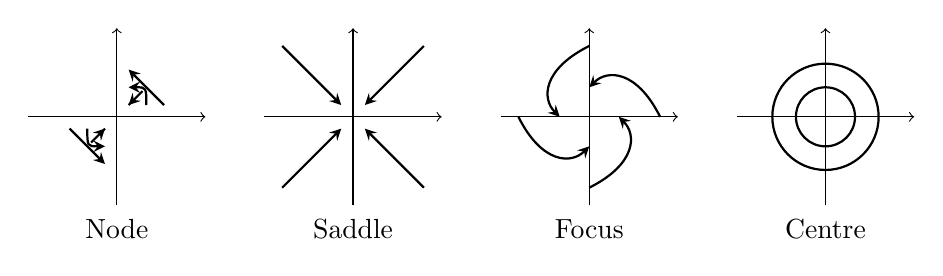
\begin{tikzpicture}[scale=0.75, arr/.style={->, thick, >=stealth}]
  % node
  \begin{scope}[shift={(0,0)}]
    \draw[->] (-1.5,0)--(1.5,0); \draw[->] (0,-1.5)--(0,1.5);
    \foreach \a in {0.2,0.5,0.8} {
      \draw[arr] (\a,0.2) .. controls (0.5,0.5) .. (0.2,\a);
      \draw[arr] (-\a,-0.2) .. controls (-0.5,-0.5) .. (-0.2,-\a);
    }
    \node at (0,-1.9) {Node};
  \end{scope}
  % saddle
  \begin{scope}[shift={(4,0)}]
    \draw[->] (-1.5,0)--(1.5,0); \draw[->] (0,-1.5)--(0,1.5);
    \draw[arr] (-1.2,-1.2) -- (-0.2,-0.2);
    \draw[arr] (1.2,1.2) -- (0.2,0.2);
    \draw[arr] (-1.2,1.2) -- (-0.2,0.2);
    \draw[arr] (1.2,-1.2) -- (0.2,-0.2);
    \node at (0,-1.9) {Saddle};
  \end{scope}
  % focus
  \begin{scope}[shift={(8,0)}]
    \draw[->] (-1.5,0)--(1.5,0); \draw[->] (0,-1.5)--(0,1.5);
    \draw[arr] (1.2,0) .. controls (0.8,0.8) and (0.3,0.8) .. (0,0.5);
    \draw[arr] (0,1.2) .. controls (-0.8,0.8) and (-0.8,0.3) .. (-0.5,0);
    \draw[arr] (-1.2,0) .. controls (-0.8,-0.8) and (-0.3,-0.8) .. (0,-0.5);
    \draw[arr] (0,-1.2) .. controls (0.8,-0.8) and (0.8,-0.3) .. (0.5,0);
    \node at (0,-1.9) {Focus};
  \end{scope}
  % centre
  \begin{scope}[shift={(12,0)}]
    \draw[->] (-1.5,0)--(1.5,0); \draw[->] (0,-1.5)--(0,1.5);
    \draw[arr] (0,0) circle (0.9);
    \draw[arr] (0,0) circle (0.5);
    \node at (0,-1.9) {Centre};
  \end{scope}
\end{tikzpicture}
\caption{The four classes of phase portrait of a planar linear system with constant coefficients: node, saddle, focus and centre.}
\label{fig:phase_portrait_classification}
\end{figure}

\begin{proof}
\textbf{(i) Node}: let $\lambda_1, \lambda_2 > 0$ (the negative case is similar). After a linear change of coordinates the system becomes $\dot{u} = \lambda_1 u$, $\dot{v} = \lambda_2 v$, with solution $u(t) = u_0 e^{\lambda_1 t}$, $v(t) = v_0 e^{\lambda_2 t}$. Eliminating $t$ gives the orbit equation $v = C u^{\lambda_2/\lambda_1}$ (when $v_0 \neq 0$). As $t \to \infty$, all orbits tend to the origin; as $t \to -\infty$, the orbits move away from the origin. The orbits are parabolic in shape (or straight lines, when $u_0 = 0$ or $v_0 = 0$).

\textbf{(ii) Saddle}: let $\lambda_1 > 0 > \lambda_2$. The solution is $u = u_0 e^{\lambda_1 t}$, $v = v_0 e^{\lambda_2 t}$. As $t \to \infty$, $u \to \infty$ whilst $v \to 0$; as $t \to -\infty$, $u \to 0$ whilst $v \to \infty$. The orbits are hyperbolic in shape.

\textbf{(iii) Focus}: let $\lambda = \alpha \pm i\beta$ with $\alpha, \beta \neq 0$. In polar coordinates the solution is $r(t) = r_0 e^{\alpha t}$, $\theta(t) = \theta_0 + \beta t$. The orbits are spirals: for $\alpha > 0$ the spiral is outward (an unstable focus), and for $\alpha < 0$ it is inward (a stable focus).

\textbf{(iv) Centre}: $\lambda = \pm i\beta$. The solution is $r(t) = r_0$ (a constant), $\theta(t) = \theta_0 + \beta t$. The orbits are concentric circles (or concentric ellipses under a general linear change of coordinates); they are closed but not isolated (they are not limit cycles).
\end{proof}

\begin{definition}[Stability of an Equilibrium Point]\label{def:equilibrium_stability}
Let $\mathbf{y}^*$ be an equilibrium point of an autonomous system. Its stability is determined by the eigenvalues of the Jacobi matrix $J = D\mathbf{F}(\mathbf{y}^*)$:
\begin{enumerate}[label=(\roman*)]
    \item all eigenvalues have negative real part: \textbf{asymptotically stable} (an attractor).
    \item some eigenvalue has positive real part: \textbf{unstable}.
    \item all eigenvalues have zero real part: the linearised system is of centre type, and higher-order analysis is required.
\end{enumerate}
If all eigenvalues have non-zero real part, the equilibrium point is called a \textbf{hyperbolic equilibrium point}.
\end{definition}

\begin{theorem}[Hartman--Grobman Theorem]\label{thm:hartman_grobman}
Let $\mathbf{y}^*$ be a hyperbolic equilibrium point of an autonomous system. Then there is a neighbourhood of $\mathbf{y}^*$ in which the original nonlinear system is topologically conjugate to the linearised system $\frac{d\mathbf{z}}{dt} = J\mathbf{z}$.
\end{theorem}

\begin{proof}
\textbf{The proof lies beyond the scope of this chapter}. This is a deep theorem in dynamical systems theory, whose complete proof requires topological methods on manifolds (see Perko, \textit{Differential Equations and Dynamical Systems}, 3rd ed., Springer, 2001, \S{}2.8). The core idea is to construct a homeomorphism $H$ such that $H \circ \Phi_t = e^{Jt} \circ H$ holds in a neighbourhood of the equilibrium point, where $\Phi_t$ is the nonlinear flow and $e^{Jt}$ is the linearised flow. The construction uses the contraction mapping principle to solve a functional equation in a function space.
\end{proof}

\begin{definition}[Limit Cycle]\label{def:limit_cycle}
A \textbf{limit cycle} is an isolated periodic orbit of an autonomous nonlinear system. A limit cycle is the periodic realisation, in a dissipative system, of the \textbf{dynamic balance between volume contraction and expansion}: the closure of the orbit is maintained by the dynamic balance between energy input and dissipation, rather than being guaranteed by a global conserved quantity.
\end{definition}

\begin{theorem}[Poincaré--Bendixson Theorem]\label{thm:poincare_bendixson}
Let $\frac{dy}{dt} = \mathbf{F}(y)$ be a planar autonomous system whose positively bounded orbits do not tend to any equilibrium point. Then the $\omega$-limit set of such an orbit must be a limit cycle.
\end{theorem}

\begin{proof}
\textbf{The proof lies beyond the scope of this chapter}. This is a classical result in the theory of planar dynamical systems (see Perko, \textit{Differential Equations and Dynamical Systems}, 3rd ed., Springer, 2001, \S{}3.7). The key to the proof is that in the plane a closed curve (a Jordan curve) divides the plane into an inside and an outside, and orbits cannot self-intersect (by the uniqueness theorem), so the $\omega$-limit set has a special topological structure. If the $\omega$-limit set contains no equilibrium point, then it must be a closed orbit.
\end{proof}

\begin{example}[van der Pol Oscillator---a Limit Cycle of Self-Excited Oscillation]\label{ex:van_der_pol}
The van der Pol equation $\ddot{x} + \mu(x^2-1)\dot{x} + x = 0$ (with $\mu > 0$). When $|x| < 1$ the damping is negative (energy is injected); when $|x| > 1$ the damping is positive (energy is dissipated). The system has a unique stable limit cycle.
\end{example}

\begin{example}[Duffing Oscillator---Nonlinear Resonance under Periodic Driving]\label{ex:duffing}
The Duffing equation $\ddot{x} + \delta \dot{x} + \alpha x + \beta x^3 = \gamma \cos \omega t$. In the $\gamma$-$\omega$ parameter plane there are Arnold tongues.
\end{example}

\subsection{Conservation Laws and First Integrals}\label{sec:first_integrals}

\begin{definition}[First Integral]\label{def:first_integral}
Let $\frac{dy}{dt} = \mathbf{F}(y)$ be an autonomous system. A function $I: \mathbb{R}^n \to \mathbb{R}$ is called a \textbf{first integral} if $I(y(t))$ is constant along every solution curve $y(t)$---that is, if $\frac{d}{dt} I(y(t)) = \nabla I(y) \cdot \mathbf{F}(y) = 0$.

A first integral is precisely a \textbf{conserved quantity} of the differential equation.
\end{definition}

\begin{proposition}[First Integrals and Orbit Constraints]\label{prop:first_integral_orbit}
If a system has $k$ independent first integrals $I_1, \dots, I_k$, then its solutions are constrained to an $(n-k)$-dimensional invariant manifold. When $k = n-1$, the orbit is completely determined by the first integrals.
\end{proposition}

\begin{proof}
The independent first integrals give the level set
\[
\mathcal{M} = \{y \in \mathbb{R}^n : I_1(y) = c_1, \dots, I_k(y) = c_k\}.
\]
By the implicit function theorem (when $\nabla I_1, \dots, \nabla I_k$ are linearly independent), $\mathcal{M}$ is a submanifold of dimension $n-k$. Solution curves always lie on $\mathcal{M}$ (because each $I_j$ is constant along solution curves), so $\mathcal{M}$ is an invariant manifold. When $k = n-1$, $\mathcal{M}$ is a $1$-dimensional manifold and the solution curve is completely determined by $\mathcal{M}$ (the orbit is precisely a connected component of $\mathcal{M}$).
\end{proof}

\begin{proposition}[Noether-Type Correspondence---a One-Parameter Symmetry Group Yields a First Integral]\label{prop:noether_ode}
Let the system $\frac{dy}{dt} = \mathbf{F}(y)$ be invariant under the one-parameter transformation group $\{\phi_s\}_{s \in \mathbb{R}}$, that is, $\phi_s \circ \Phi_t = \Phi_t \circ \phi_s$ for all $s, t$ (where $\Phi_t$ is the flow of the system). Let $\xi$ be the infinitesimal generator of $\phi_s$ at $s=0$, that is, $\xi(y) = \frac{d}{ds}\big|_{s=0} \phi_s(y)$. If there is a smooth function $I: \mathbb{R}^n \to \mathbb{R}$ such that $\xi = J \nabla I$ (with $J$ a non-degenerate antisymmetric matrix, that is, a symplectic structure), then $I$ is a first integral of the system.
\end{proposition}

\begin{proof}
From the invariance $\phi_s \circ \Phi_t = \Phi_t \circ \phi_s$, differentiating with respect to $s$ at $s=0$ gives $[\xi, \mathbf{F}] = 0$, that is, the Lie bracket vanishes. If $\xi = J\nabla I$, then $\nabla I$ satisfies
\[
\frac{d}{dt} I(y(t)) = \nabla I \cdot \mathbf{F} = (J^{-1}\xi) \cdot \mathbf{F}.
\]
From $[\xi, \mathbf{F}] = 0$ and the antisymmetry of $J$ one can deduce that $\nabla I \cdot \mathbf{F} = 0$ (see Arnold, \textit{Mathematical Methods of Classical Mechanics}, 2nd ed., Springer, 1989, \S{}38, for details). Hence $I$ is a first integral.
\end{proof}

\begin{figure}[htbp]
\centering
\begin{tikzpicture}[
  box/.style={draw, rounded corners, fill=green!8, align=center, inner sep=5pt, font=\small},
  arr/.style={->, thick, >=stealth}
]
  \node[box] (sym) {One-parameter symmetry group\\$\phi_s\circ\Phi_t=\Phi_t\circ\phi_s$};
  \node[box, right=1.2cm of sym] (xi) {Infinitesimal generator\\$\xi=\frac{d}{ds}\big|_{s=0}\phi_s$};
  \node[box, right=1.2cm of xi] (J) {Symplectic structure\\$\xi=J\nabla I$};
  \node[box, below=1.0cm of J] (cons) {First integral\\$\frac{d}{dt}I(y(t))=0$};
  \draw[arr] (sym) -- (xi);
  \draw[arr] (xi) -- (J);
  \draw[arr] (J) -- (cons);
\end{tikzpicture}
\caption{Noether-type correspondence: a continuous symmetry yields a first integral.}
\label{fig:noether_ode}
\end{figure}

\begin{example}[First Integrals in Classical Mechanics]\label{ex:classical_first_integrals}
\begin{enumerate}[label=(\roman*)]
    \item \textbf{Conservation of energy}: in a conservative force field the total mechanical energy $E = \frac{1}{2}m\|\dot{\mathbf{r}}\|^2 + V(\mathbf{r})$ is a first integral. It corresponds to invariance under time translation.
    \item \textbf{Conservation of angular momentum}: in a central force field the angular momentum $\mathbf{L} = m \mathbf{r} \times \dot{\mathbf{r}}$ is a first integral. It corresponds to rotational symmetry.
    \item \textbf{Conservation of momentum}: when no external force acts in a given direction, the momentum component in that direction is a first integral. It corresponds to spatial translation symmetry.
\end{enumerate}
\end{example}

\section{Periodic-Coefficient Differential Equations and Floquet Theory}\label{sec:floquet}

\begin{definition}[Linear System with Periodic Coefficients]\label{def:periodic_coefficient_system}
Let $A(t)$ satisfy $A(t+T) = A(t)$ for all $t$. The system $\frac{dy}{dt} = A(t) y$ is called a \textbf{linear system with periodic coefficients}.
\end{definition}

\begin{theorem}[Floquet's Theorem]\label{thm:floquet}
Let $\Phi(t)$ be a fundamental solution matrix of a linear system with periodic coefficients. Then there exist a non-singular $T$-periodic matrix $P(t)$ and a constant matrix $B$ such that
\[
\Phi(t) = P(t) e^{Bt}.
\]
The matrix $M = \Phi(T, 0)$ is called the \textbf{monodromy matrix}, and its eigenvalues $\rho_1, \dots, \rho_n$ are called the \textbf{Floquet multipliers}.
\end{theorem}

\begin{figure}[htbp]
\centering
\begin{tikzpicture}[
  box/.style={draw, rounded corners, align=center, inner sep=6pt, font=\small},
  arr/.style={->, thick, >=stealth}
]
  \node[box, fill=blue!8] (per) {Periodic-coefficient system\\$\dot y=A(t)y,\;A(t+T)=A(t)$};
  \node[box, fill=orange!12, right=1.5cm of per] (M) {Monodromy matrix\\$M=\Phi(T,0)$};
  \node[box, fill=green!12, right=1.5cm of M] (rho) {Floquet multipliers\\$\rho=e^{\lambda T}$};
  \node[box, fill=red!8, below=1.2cm of rho] (stab) {Stability criterion\\$|\rho|<1$ decay; $|\rho|=1$ periodic/rotation};
  \draw[arr] (per) -- (M);
  \draw[arr] (M) -- (rho);
  \draw[arr] (rho) -- (stab);
\end{tikzpicture}
\caption{Logical chain of Floquet theory: periodic-coefficient system $\to$ monodromy matrix $\to$ Floquet multipliers $\to$ stability and periodic solutions.}
\label{fig:floquet_flow}
\end{figure}

\begin{proof}
Define $M = \Phi(T, 0)$. By the periodicity $A(t+T) = A(t)$, verify that $\Phi(t+T, 0)$ is also a fundamental solution matrix: $\frac{d}{dt}\Phi(t+T, 0) = A(t+T)\Phi(t+T, 0) = A(t)\Phi(t+T, 0)$, and $\Phi(T, 0) = M$ is non-singular. Hence $\Phi(t+T, 0) = \Phi(t, 0) M$ (two fundamental solution matrices differ by a constant matrix factor).

Define $B = \frac{1}{T} \log M$ (the matrix logarithm exists because $M$ is non-singular; if $M$ has a negative real eigenvalue, $\log M$ may be a complex matrix, in which case $B$ is a complex matrix and $P(t)$ is a complex $T$-periodic matrix). Define $P(t) = \Phi(t, 0) e^{-Bt}$. Verify that $P(t)$ is $T$-periodic:
\[
P(t+T) = \Phi(t+T, 0) e^{-B(t+T)} = \Phi(t, 0) M e^{-BT} e^{-Bt} = \Phi(t, 0) e^{-Bt} = P(t),
\]
where we used $e^{-BT} = e^{-\log M} = M^{-1}$. Hence $\Phi(t) = P(t) e^{Bt}$.
\end{proof}

\begin{corollary}[Floquet Multipliers and the Stability of Periodic Solutions]\label{cor:floquet_stability}
\begin{enumerate}[label=(\roman*)]
    \item $\rho = 1$: the system has a $T$-periodic solution.
    \item $\rho = -1$: the system has a $2T$-periodic solution (period-doubling bifurcation).
    \item $\rho = e^{i 2\pi p/q}$: the system has a $qT$-periodic solution.
    \item all $|\rho_i| < 1$ (with $i \neq 1$ and $\rho_1 = 1$): this periodic solution is asymptotically stable.
\end{enumerate}
\end{corollary}

\begin{proof}
The relation between an eigenvalue $\rho$ of the monodromy matrix and the Floquet exponent $\lambda$ is $\rho = e^{\lambda T}$ (because $M = e^{BT}$ and the eigenvalues of $B$ are $\lambda$).

(i) $\rho = 1 \iff \lambda = 2\pi i k/T$ ($k \in \mathbb{Z}$). The corresponding solution is unchanged under the time translation $T$, that is, it is a $T$-periodic solution.

(ii) $\rho = -1 \iff \lambda = \pi i(2k+1)/T$. The corresponding solution is unchanged under the time translation $2T$ ($e^{\lambda \cdot 2T} = e^{2\pi i(2k+1)} = 1$), that is, it is a $2T$-periodic solution.

(iii) $\rho = e^{2\pi i p/q}$ (with $p/q$ in lowest terms) $\iff \lambda T = 2\pi i p/q + 2\pi i k$. The corresponding solution is unchanged under the time translation $qT$, that is, it is a $qT$-periodic solution.

(iv) $|\rho| < 1 \iff \operatorname{Re}\lambda < 0$. The corresponding Floquet component decays exponentially. If all $|\rho_i| < 1$ except $\rho_1 = 1$, then every perturbative component of this periodic solution decays, and the periodic solution is asymptotically stable.
\end{proof}

\begin{proposition}[Correspondence between Floquet Multipliers and the Three Operators]\label{prop:floquet_operator}
The eigenvalue decomposition of the monodromy matrix $M$ corresponds to three operators:
\begin{enumerate}[label=(\roman*)]
    \item \textbf{Rotation part}: the multipliers with $|\rho_i| = 1$ correspond to pure rotation.
    \item \textbf{Scaling part}: the multipliers with $|\rho_i| \neq 1$ correspond to scaling.
    \item \textbf{Translation part}: the period $T$ itself carries the translation symmetry.
\end{enumerate}
\end{proposition}

\begin{proof}
By the proof of Corollary \ref{cor:floquet_stability}, $|\rho| = 1 \iff \operatorname{Re}\lambda = 0$, and the Floquet component neither grows nor decays but rotates purely on an invariant torus. $|\rho| \neq 1 \iff \operatorname{Re}\lambda \neq 0$, and the Floquet component grows or decays exponentially, its ratio being the scaling factor of volume. The period $T$ is the parameter of the time-translation symmetry.
\end{proof}

\begin{example}[Hill's Equation---a Periodically Driven Oscillator]\label{ex:hill_equation}
The Hill equation $\ddot{y} + p(t) y = 0$ (with $p(t+T) = p(t)$). When $p(t) = \omega_0^2 + \varepsilon \cos \omega t$ it reduces to the Mathieu equation. Written as $\dot y=A(t)y$ the Hill equation has $\operatorname{tr}A\equiv0$, so Liouville's formula (Proposition \ref{prop:liouville_formula}) gives $\det\Phi(T,0)=1$; hence its Floquet multipliers satisfy $\rho_1 \rho_2 = 1$.
\end{example}

\begin{example}[Mathieu's Equation and Parametric Resonance]\label{ex:mathieu}
The Mathieu equation $\ddot{y} + (\delta + \varepsilon \cos 2t) y = 0$ (period $T = \pi$). In the $\delta$-$\varepsilon$ parameter plane, stable and unstable regions alternate.
\end{example}

\section{Fundamentals of Partial Differential Equations}\label{sec:pde_basic}

\begin{definition}[Partial Differential Equation]\label{def:pde}
Let $u: \mathbb{R}^n \to \mathbb{R}$ be an unknown function. A \textbf{$k$-th order partial differential equation} is an equation involving $u$ and its partial derivatives up to order $k$.
\end{definition}

\begin{definition}[Wave Equation]\label{def:wave_equation}
The \textbf{wave equation} is
\[
\frac{\partial^2 u}{\partial t^2} - c^2 \nabla^2 u = 0.
\]
Its general solution is $u(\mathbf{x}, t) = f(\mathbf{x} \cdot \mathbf{n} - ct) + g(\mathbf{x} \cdot \mathbf{n} + ct)$.
\end{definition}

\begin{definition}[Heat Equation]\label{def:heat_equation}
The \textbf{heat equation} is
\[
\frac{\partial u}{\partial t} - \alpha \nabla^2 u = 0.
\]
Each Fourier component decays exponentially: $c_n(t) = c_n(0) e^{-\alpha (2\pi n/T)^2 t}$.
\end{definition}

\begin{definition}[Laplace's Equation]\label{def:laplace_equation}
The \textbf{Laplace equation} is $\nabla^2 u = 0$. Its solutions are called \textbf{harmonic functions}.
\end{definition}

\begin{proposition}[Fourier Method for Linear Partial Differential Equations with Constant Coefficients]\label{prop:pde_fourier_solution}
For a linear partial differential equation with constant coefficients and periodic boundary conditions, the Fourier transform converts it into an algebraic equation or an ordinary differential equation. Let $u(\mathbf{x}, t) = \sum_{\mathbf{k}} \hat{u}_{\mathbf{k}}(t) e^{i \mathbf{k} \cdot \mathbf{x}}$; the component of each wave vector $\mathbf{k}$ evolves independently.
\end{proposition}

\begin{figure}[htbp]
\centering
\begin{tikzpicture}[
  box/.style={draw, rounded corners, fill=blue!8, align=center, inner sep=5pt, font=\small},
  arr/.style={->, thick, >=stealth}
]
  \node[box] (pde) {Linear PDE with constant coefficients\\periodic boundary};
  \node[box, right=1.2cm of pde] (fourier) {Fourier expansion\\$u=\sum_{\mathbf k}\hat u_{\mathbf k}(t)e^{i\mathbf k\cdot\mathbf x}$};
  \node[box, right=1.2cm of fourier] (ode) {Independent ODE for each mode\\$\hat u_{\mathbf k}(t)$};
  \node[box, below=1.0cm of ode] (sol) {Composite solution\\$u(\mathbf x,t)=\sum_{\mathbf k}\hat u_{\mathbf k}(t)e^{i\mathbf k\cdot\mathbf x}$};
  \draw[arr] (pde) -- (fourier);
  \draw[arr] (fourier) -- (ode);
  \draw[arr] (ode) -- (sol);
\end{tikzpicture}
\caption{The Fourier method for linear partial differential equations with constant coefficients: spatial derivatives become multiplication and the modes of each wave vector evolve independently.}
\label{fig:pde_fourier_flow}
\end{figure}

\begin{proof}
Substitute $u(\mathbf{x}, t) = \sum_{\mathbf{k}} \hat{u}_{\mathbf{k}}(t) e^{i \mathbf{k} \cdot \mathbf{x}}$ into the partial differential equation. For a linear operator $\mathcal{L}(\partial_{\mathbf{x}}, \partial_t)$ with constant coefficients, its action on $e^{i\mathbf{k}\cdot\mathbf{x}}$ is $\mathcal{L}(i\mathbf{k}, \partial_t) e^{i\mathbf{k}\cdot\mathbf{x}}$ (the Fourier transform converts the spatial derivative $\partial_{x_j}$ into multiplication by $ik_j$). By the orthogonality of the Fourier basis, the various $\mathbf{k}$ components are independent, and each $\hat{u}_{\mathbf{k}}(t)$ satisfies an ordinary differential equation.
\end{proof}

\begin{example}[Fourier Method for the Heat Equation]\label{ex:heat_fourier}
For $\frac{\partial u}{\partial t} = \alpha \nabla^2 u$, substituting the Fourier series gives $\frac{d \hat{u}_{\mathbf{k}}}{dt} = -\alpha |\mathbf{k}|^2 \hat{u}_{\mathbf{k}}$, whose solution is $\hat{u}_{\mathbf{k}}(t) = \hat{u}_{\mathbf{k}}(0) e^{-\alpha |\mathbf{k}|^2 t}$.
\end{example}

\begin{example}[Fourier Method for the Wave Equation]\label{ex:wave_fourier}
For $\frac{\partial^2 u}{\partial t^2} = c^2 \nabla^2 u$, substituting the Fourier series gives $\frac{d^2 \hat{u}_{\mathbf{k}}}{dt^2} = -c^2 |\mathbf{k}|^2 \hat{u}_{\mathbf{k}}$, whose solution is $\hat{u}_{\mathbf{k}}(t) = A_{\mathbf{k}} e^{i c |\mathbf{k}| t} + B_{\mathbf{k}} e^{-i c |\mathbf{k}| t}$.
\end{example}

\section{Green's Functions and Integral Equations}\label{sec:green_integral}

\begin{definition}[Green's Function]\label{def:green_function}
For a linear differential operator $\mathcal{L}$, its \textbf{Green's function} $G(\mathbf{x}, \boldsymbol{\xi})$ satisfies
\[
\mathcal{L} G(\mathbf{x}, \boldsymbol{\xi}) = \delta(\mathbf{x} - \boldsymbol{\xi}).
\]
The solution of the inhomogeneous equation $\mathcal{L} u = f$ is
\[
u(\mathbf{x}) = \int G(\mathbf{x}, \boldsymbol{\xi}) f(\boldsymbol{\xi}) d\boldsymbol{\xi} = (G * f)(\mathbf{x}).
\]
\end{definition}

\begin{remark}[Existence of Green's Functions]\label{rem:green_existence}
A Green's function exists if and only if the homogeneous equation $\mathcal{L} u = 0$ (under the given boundary conditions) has only the zero solution. This is a direct corollary of the Fredholm alternative theorem (Theorem \ref{thm:fredholm_alternative}): if the kernel of $\mathcal{L}$ is non-trivial, then $\mathcal{L}$ is not invertible and the Green's function does not exist.
\end{remark}

\begin{example}[Fundamental Solution of the Laplace Operator]\label{ex:laplace_green}
The fundamental solution of the three-dimensional Laplace operator is $G(\mathbf{x}) = -\frac{1}{4\pi |\mathbf{x}|}$ (satisfying $\nabla^2 G = \delta(\mathbf{x})$). This agrees exactly with the inverse-square law.
\end{example}

\begin{example}[Fundamental Solution of the Heat Operator]\label{ex:heat_green}
The fundamental solution of the one-dimensional heat operator is $G(x, t) = \frac{1}{\sqrt{4\pi\alpha t}} e^{-x^2/(4\alpha t)}$. The solution of the heat equation is the convolution of the initial condition with the Gaussian kernel.
\end{example}

\begin{definition}[Fredholm Integral Equation]\label{def:fredholm_integral_equation}
The \textbf{Fredholm integral equation of the second kind} is
\[
u(x) - \lambda \int_a^b K(x, y) u(y) \, dy = f(x).
\]
When $K(x, y) = K(x-y)$ (a convolution kernel), the Fredholm equation can be diagonalised by the Fourier transform.
\end{definition}

\begin{definition}[Volterra Integral Equation]\label{def:volterra_integral_equation}
The \textbf{Volterra integral equation of the second kind} is
\[
u(x) - \lambda \int_a^x K(x, y) u(y) \, dy = f(x).
\]
A Volterra equation corresponds to causal accumulation---the integral depends only on past values.
\end{definition}

\begin{theorem}[Fredholm Alternative Theorem]\label{thm:fredholm_alternative}
For a Fredholm integral equation with continuous kernel, exactly one of the following two alternatives holds:
\begin{enumerate}[label=(\roman*)]
    \item for every $f$ the equation has a unique solution.
    \item the homogeneous equation $u - \lambda Ku = 0$ has a non-zero solution.
\end{enumerate}
\end{theorem}

\begin{proof}
\textbf{The proof lies beyond the scope of this chapter}. This is a fundamental theorem of the spectral theory of compact operators (see Conway, \textit{A Course in Functional Analysis}, 2nd ed., Springer, 1990, \S{}VII.6). The core fact is that an integral operator $K$ with continuous kernel is compact, and its spectrum consists of at most countably many eigenvalues tending to zero. If $\lambda^{-1}$ is not an eigenvalue of $K$, then $(I - \lambda K)$ is invertible and the equation has a unique solution; if $\lambda^{-1}$ is an eigenvalue, then the homogeneous equation has a non-zero solution.
\end{proof}

\begin{proposition}[Equivalence of Integral and Differential Equations]\label{prop:integral_differential_equivalence}
An initial-value problem for an ordinary differential equation with initial conditions is equivalent to a Volterra integral equation; a boundary-value problem for an ordinary differential equation with boundary conditions is equivalent to a Fredholm integral equation.
\end{proposition}

\begin{figure}[htbp]
\centering
\begin{tikzpicture}[
  box/.style={draw, rounded corners, align=center, inner sep=5pt, font=\small},
  arr/.style={->, thick, >=stealth}
]
  \node[box, fill=blue!8] (ivp) {Initial-value problem\\$\dot y=F(t,y),y(t_0)=y_0$};
  \node[box, fill=orange!12, right=1.5cm of ivp] (vol) {Volterra integral equation\\$y=y_0+\int_{t_0}^t F(s,y(s))ds$};
  \node[box, fill=green!12, below=1.2cm of ivp] (bvp) {Boundary-value problem\\$\mathcal L u=f$ + boundary conditions};
  \node[box, fill=red!8, right=1.5cm of bvp] (fred) {Fredholm integral equation\\$u-\lambda Ku=f$};
  \draw[arr] (ivp) -- (vol);
  \draw[arr] (bvp) -- (fred);
\end{tikzpicture}
\caption{The equivalence between differential and integral equations: the initial-value problem corresponds to a Volterra equation and the boundary-value problem to a Fredholm equation.}
\label{fig:integral_differential_equivalence}
\end{figure}

\begin{proof}
The initial-value problem $\frac{dy}{dt} = F(t,y)$, $y(t_0) = y_0$ is equivalent to $y(t) = y_0 + \int_{t_0}^t F(s, y(s))\,ds$---this is a Volterra equation of the second kind (the linearisation of the kernel $K(t,s) = F$). This equivalence was already established in Step 1 of the proof of Theorem \ref{thm:picard_lindelof}.

A boundary-value problem is represented by means of the Green's function (Definition \ref{def:green_function}): $u = G * f$, that is, $u(x) = \int G(x,\xi)f(\xi)d\xi$. Rewriting this in the form $u - \lambda K u = f$ (where $K$ is the integral operator corresponding to the Green's function) gives a Fredholm equation of the second kind.
\end{proof}

\section{Foundations of Complex Analysis}\label{sec:complex_analysis}

\subsection{The Algebra and Geometry of Complex Numbers}

\begin{definition}[The Field of Complex Numbers]\label{def:complex_field}
Let $\mathbb{C} = \{(a, b) : a, b \in \mathbb{R}\}$, equipped with the addition $(a,b)+(c,d) = (a+c, b+d)$ and the multiplication $(a,b)(c,d) = (ac - bd, ad + bc)$. Write $i = (0,1)$; then every complex number can be written as $z = a + bi$.
\end{definition}

\begin{property}[Basic Properties of the Field of Complex Numbers]\label{prop:complex_field_props}
\begin{enumerate}[label=(\roman*)]
    \item $(\mathbb{C}, +, \times)$ is a field, with $0$ the additive identity and $1$ the multiplicative identity.
    \item $i^2 = -1$, and $\mathbb{C} = \mathbb{R}[i] \cong \mathbb{R}[x]/(x^2+1)$.
    \item \textbf{Conjugation}: $\overline{a+bi} = a - bi$, satisfying $\overline{z+w} = \bar z + \bar w$ and $\overline{zw} = \bar z \bar w$.
    \item \textbf{Modulus}: $|z| = \sqrt{z\bar z} = \sqrt{a^2+b^2}$, satisfying $|zw| = |z||w|$ (multiplicativity) and $|z+w| \le |z|+|w|$ (the triangle inequality).
    \item \textbf{Polar form}: a non-zero $z = re^{i\theta}$, where $r = |z| > 0$ and $\theta = \arg z \in \mathbb{R}/(2\pi\mathbb{Z})$ is the argument.
\end{enumerate}
\end{property}

\begin{definition}[Three Centres of Symmetry in the Complex Plane]\label{def:complex_centres}
The complex plane has three intrinsic centres of symmetry:
\begin{enumerate}[label=(\roman*)]
    \item $0$ (the additive identity): the fixed point of the additive reflection $z \mapsto -z$.
    \item $1$ (the multiplicative identity): one of the fixed points of multiplicative inversion $\sigma_1(z) = 1/z$.
    \item $i$ (the imaginary unit): the \textbf{centre of symmetry} of the $i$-involution $\sigma_i(z) = i z^{-1}$ (the composite centre of $\sigma_i = R_{\pi/2}\circ\sigma_1$); the fixed points of $\sigma_i$ are $z = \pm\frac{\sqrt2}{2}(1+i)$, and $i^4 = 1$ generates $C_4$.
\end{enumerate}
\end{definition}

\subsection{Limits of Complex Sequences and Complex Functions}

\begin{definition}[Limit of a Complex Sequence]\label{def:complex_seq_limit}
Let $\{z_n\}$ be a complex sequence and $L \in \mathbb{C}$. We say that $\lim z_n = L$ if
\[
\forall \varepsilon > 0,\; \exists N \in \mathbb{N},\; \forall n > N,\; |z_n - L| < \varepsilon.
\]
\end{definition}

\begin{proposition}[Necessary and Sufficient Condition for Convergence of a Complex Sequence]\label{prop:complex_seq_convergence}
A complex sequence $\{z_n\}$ converges to $L = a+bi$ if and only if its real and imaginary parts converge separately.
\end{proposition}

\begin{proof}
Let $z_n = x_n + iy_n$ and $L = a + bi$.

\textbf{Necessity}: if $z_n \to L$, then for any $\varepsilon > 0$ there is $N$ such that $|z_n - L| < \varepsilon$ whenever $n > N$. Since
\[
|x_n - a| \le \sqrt{(x_n-a)^2 + (y_n-b)^2} = |z_n - L| < \varepsilon,
\]
we have $x_n \to a$. Similarly $y_n \to b$.

\textbf{Sufficiency}: if $x_n \to a$ and $y_n \to b$, then for any $\varepsilon > 0$ there are $N_1, N_2$ such that $|x_n - a| < \varepsilon/\sqrt{2}$ whenever $n > N_1$ and $|y_n - b| < \varepsilon/\sqrt{2}$ whenever $n > N_2$. Take $N = \max\{N_1, N_2\}$; then for $n > N$,
\[
|z_n - L| = \sqrt{(x_n-a)^2 + (y_n-b)^2} < \sqrt{\varepsilon^2/2 + \varepsilon^2/2} = \varepsilon.
\]
\end{proof}

\begin{property}[The Cauchy Criterion and Completeness for Sequences of Complex Numbers]\label{prop:complex_cauchy}
$\mathbb{C}$ is complete: a complex sequence converges if and only if it is a Cauchy sequence. That is, $\{z_n\}$ converges $\iff$ for any $\varepsilon > 0$ there is $N$ such that $|z_m - z_n| < \varepsilon$ whenever $m, n > N$.
\end{property}

\begin{proof}
($\Rightarrow$) If $z_n \to L$, then $|z_m - z_n| \le |z_m - L| + |L - z_n| \to 0$.

($\Leftarrow$) If $\{z_n\}$ is a Cauchy sequence, then $|x_m - x_n| \le |z_m - z_n|$ shows that $\{x_n\}$ is a Cauchy sequence of real numbers, which converges to $a$ by the completeness of $\mathbb{R}$; similarly $\{y_n\}$ converges to $b$. By \cref{prop:complex_seq_convergence}, $z_n \to a+bi$.
\end{proof}

\begin{definition}[Limit and Continuity of a Complex-Valued Function]\label{def:complex_limit}
Let $f: \mathbb{C} \supseteq D \to \mathbb{C}$. We say that $\lim_{z\to z_0} f(z) = L$ if
\[
\forall \varepsilon > 0,\; \exists \delta > 0,\; \forall z \in D,\; 0 < |z - z_0| < \delta \implies |f(z) - L| < \varepsilon.
\]
If $\lim_{z\to z_0} f(z) = f(z_0)$, then $f$ is said to be continuous at $z_0$.
\end{definition}

\subsection{Complex Derivatives and Analytic Functions}\label{sec:analytic_functions}

\begin{definition}[Complex Derivative]\label{def:complex_derivative}
Let $f: \mathbb{C} \supseteq D \to \mathbb{C}$ and $z_0 \in D$. If the limit
\[
f'(z_0) := \lim_{h \to 0} \frac{f(z_0 + h) - f(z_0)}{h}
\]
exists and is finite, then $f$ is said to be \textbf{complex differentiable} at $z_0$. Here $h \in \mathbb{C}$ may tend to $0$ along an arbitrary path.
\end{definition}

\begin{definition}[Analytic Function]\label{def:analytic_function}
If $f$ is complex differentiable at every point of an open set $U \subseteq \mathbb{C}$, then $f$ is said to be \textbf{analytic} (or \textbf{holomorphic}) on $U$. If $f$ is analytic in some neighbourhood of $z_0$, then $f$ is said to be analytic at $z_0$.
\end{definition}

\begin{definition}[Entire Function]\label{def:entire_function}
A function analytic on the whole of $\mathbb{C}$ is called an \textbf{entire function}. For example, $e^z$, $\sin z$, $\cos z$ and all polynomials are entire functions.
\end{definition}

\begin{theorem}[Cauchy--Riemann Equations]\label{thm:cauchy_riemann}
Let $f(z) = u(x,y) + i v(x,y)$. If $f$ is complex differentiable at $z_0$, then
\[
\frac{\partial u}{\partial x} = \frac{\partial v}{\partial y}, \quad \frac{\partial u}{\partial y} = -\frac{\partial v}{\partial x}.
\]
\end{theorem}

\begin{proof}
Consider $h \to 0$ along the real axis ($h = \Delta x$, $\Delta y = 0$):
\[
f'(z_0) = \lim_{\Delta x \to 0} \frac{f(x_0+\Delta x, y_0) - f(x_0, y_0)}{\Delta x} = \frac{\partial u}{\partial x}(x_0,y_0) + i\frac{\partial v}{\partial x}(x_0,y_0).
\]
Along the imaginary axis ($h = i\Delta y$, $\Delta x = 0$):
\[
f'(z_0) = \lim_{\Delta y \to 0} \frac{f(x_0, y_0+\Delta y) - f(x_0, y_0)}{i\Delta y} = \frac{1}{i}\left(\frac{\partial u}{\partial y} + i\frac{\partial v}{\partial y}\right) = \frac{\partial v}{\partial y} - i\frac{\partial u}{\partial y}.
\]
Since $f$ is complex differentiable, the two limits must be equal. Comparing real and imaginary parts:
\[
\frac{\partial u}{\partial x} = \frac{\partial v}{\partial y}, \qquad \frac{\partial v}{\partial x} = -\frac{\partial u}{\partial y}.
\]
\end{proof}

\begin{figure}[htbp]
\centering
\begin{tikzpicture}[
  box/.style={draw, rounded corners, align=center, inner sep=5pt, font=\small},
  arr/.style={->, thick, >=stealth}
]
  \node[box, fill=blue!8] (diff) {Complex differentiable\\$f'(z_0)$ exists};
  \node[box, fill=orange!12, right=1.2cm of diff] (cr) {Cauchy--Riemann equations\\$u_x=v_y,\;u_y=-v_x$};
  \node[box, fill=green!12, right=1.2cm of cr] (analytic) {Analytic/holomorphic\\complex differentiable everywhere on an open set};
  \node[box, fill=red!8, below=1.0cm of cr] (harmonic) {Real and imaginary parts harmonic\\$\nabla^2u=\nabla^2v=0$};
  \draw[arr] (diff) -- (cr);
  \draw[arr] (cr) -- (analytic);
  \draw[arr] (cr) -- (harmonic);
\end{tikzpicture}
\caption{The relations between complex differentiability, the Cauchy--Riemann equations, analyticity and harmonicity.}
\label{fig:cr_analytic_harmonic}
\end{figure}

\begin{remark}[Cauchy--Riemann Equations and Vanishing Curl]\label{rem:cr_curl_zero}
Consider the vector field $\mathbf{F} = (u, -v)$. Its two-dimensional curl is
\[
\frac{\partial(-v)}{\partial x} - \frac{\partial u}{\partial y} = -\frac{\partial v}{\partial x} - \frac{\partial u}{\partial y} = 0
\]
(by the Cauchy--Riemann equations). Hence \textbf{an analytic function corresponds to an irrotational field}. Similarly, the divergence of the vector field $\mathbf{G} = (u, v)$ is $\partial u/\partial x + \partial v/\partial y = 2\partial u/\partial x$, which is in general non-zero. This structure of analytic functions is the meeting point of complex analysis and vector analysis.
\end{remark}

\begin{corollary}[The Real and Imaginary Parts of an Analytic Function are Harmonic]\label{cor:harmonic_parts}
If $f = u + iv$ is analytic on an open set $U$, then both $u$ and $v$ are harmonic functions:
\[
\nabla^2 u = 0, \qquad \nabla^2 v = 0.
\]
Conversely, if $u$ is harmonic on a simply connected domain, then there exists its \textbf{harmonic conjugate} $v$ such that $u + iv$ is analytic.
\end{corollary}

\begin{proof}
By the Cauchy--Riemann equations $u_x = v_y$, $u_y = -v_x$, if $f$ is twice continuously differentiable (which will be guaranteed automatically by Cauchy's integral formula in \cref{thm:cauchy_integral_formula}), then
\[
u_{xx} = (v_y)_x = v_{yx} = v_{xy} = (-u_y)_y = -u_{yy},
\]
so $u_{xx} + u_{yy} = 0$. Similarly $v$ is harmonic.
\end{proof}

\begin{proposition}[Periodicity and Derivative of the Complex Exponential Function]\label{prop:complex_exp_periodicity}
$f(z) = e^z = e^x(\cos y + i\sin y)$ is analytic on the whole complex plane, $f'(z) = e^z$, and $e^{z + 2\pi i} = e^z$.
\end{proposition}

\begin{proof}
\textbf{Derivative}: from $e^z = e^x(\cos y + i\sin y)$, verify the Cauchy--Riemann equations: $u = e^x\cos y$, $v = e^x\sin y$. $\frac{\partial u}{\partial x} = e^x\cos y$ and $\frac{\partial v}{\partial y} = e^x\cos y$, which are equal; $\frac{\partial u}{\partial y} = -e^x\sin y$ and $-\frac{\partial v}{\partial x} = -e^x\sin y$, which are equal. By the Cauchy--Riemann equations, $e^z$ is complex differentiable, and $f'(z) = \frac{\partial u}{\partial x} + i\frac{\partial v}{\partial x} = e^x\cos y + ie^x\sin y = e^z$.

\textbf{Periodicity}: $e^{z+2\pi i} = e^x e^{i(y+2\pi)} = e^x e^{iy} e^{2\pi i} = e^z$, because $e^{2\pi i} = \cos(2\pi) + i\sin(2\pi) = 1$.
\end{proof}

\begin{example}[Definitions of the Complex Elementary Functions]\label{ex:elementary_complex_functions}
\begin{enumerate}[label=(\roman*)]
    \item $\sin z = \dfrac{e^{iz} - e^{-iz}}{2i}$, $\cos z = \dfrac{e^{iz} + e^{-iz}}{2}$. Both are entire functions, with periodicity $2\pi$.
    \item $\tan z = \sin z / \cos z$ is analytic where $\cos z \neq 0$; its zeros are $\{z = \pi/2 + k\pi\}$.
    \item $\log z = \ln|z| + i\arg z$ is a multi-valued function; after taking the principal branch $\operatorname{Log}$ it is analytic on $\mathbb{C} \setminus (-\infty, 0]$.
    \item $z^\alpha = e^{\alpha \operatorname{Log} z}$ (with $\alpha \notin \mathbb{Z}$) is a multi-valued function, and its zeros and poles depend on $\alpha$.
\end{enumerate}
\end{example}

\section{Cauchy's Integral Theory}\label{sec:cauchy_theory}

\begin{lemma}[The Plane Green's Theorem (Forward Reference)]\label{lem:green_forward}
Let $P, Q \in C^1(\overline{D_\gamma})$, where $\gamma$ is a piecewise smooth simple closed curve and $D_\gamma$ is the region it encloses. Then
\[
\oint_\gamma (P\,dx + Q\,dy) = \iint_{D_\gamma}\left( \frac{\partial Q}{\partial x} - \frac{\partial P}{\partial y} \right) dx\,dy .
\]
\textbf{An independent proof of this lemma is given in the `Vector Analysis' chapter (Theorem \ref{thm:green_plane})}. This section cites it first, which constitutes a \textbf{forward reference}: the reader may accept the conclusion for now, or follow the route free of forward dependencies according to Remark \ref{rem:cauchy_without_green}.
\end{lemma}

\begin{remark}[Two Routes to Cauchy's Integral Theorem]\label{rem:cauchy_without_green}
Theorem \ref{thm:cauchy_integral} has two standard routes of proof. The first is the \textbf{Green's theorem route} adopted in this section: the contour integral is converted into two double integrals, and the Cauchy--Riemann equations then make the integrand vanish everywhere. This route requires $f'$ to be continuous, and requires the region to have a piecewise smooth boundary (the hypotheses of Lemma \ref{lem:green_forward}). The second is \textbf{Goursat's subdivision method}: triangulate the region enclosed by the path, split the integral over the large contour into integrals over small triangles, estimate piece by piece and refine the subdivision; it requires only that $f$ be differentiable on the region, and not that $f'$ be continuous. This route \textbf{does not use Green's theorem}, and therefore avoids forward dependencies altogether. This book adopts the former, in order to stay consistent with the physical picture of `flux--circulation'; the two routes give the same conclusion.
\end{remark}

\begin{theorem}[Cauchy's Integral Theorem]\label{thm:cauchy_integral}
Let $f$ be analytic on a simply connected domain $D$, and let $\gamma$ be a closed path in $D$. Then
\[
\oint_\gamma f(z)\,dz = 0.
\]
\end{theorem}

\begin{proof}
Let $f = u + iv$ and $dz = dx + i\,dy$. Expand the contour integral into real integrals:
\[
\oint_\gamma f(z)\,dz = \oint_\gamma (u + iv)(dx + i\,dy) = \oint_\gamma (u\,dx - v\,dy) + i \oint_\gamma (v\,dx + u\,dy).
\]
By Lemma \ref{lem:green_forward} (the plane Green's theorem; for its independent proof see Theorem \ref{thm:green_plane} in the `Vector Analysis' chapter, this being a forward reference), for the closed path $\gamma$ in $D$ and the region $D_\gamma$ it encloses, taking $(P,Q) = (u,-v)$ and $(P,Q) = (v,u)$ gives respectively
\[
\oint_\gamma (u\,dx - v\,dy) = -\iint_{D_\gamma} \left( \frac{\partial v}{\partial x} + \frac{\partial u}{\partial y} \right) dx\,dy,
\]
\[
\oint_\gamma (v\,dx + u\,dy) = \iint_{D_\gamma} \left( \frac{\partial u}{\partial x} - \frac{\partial v}{\partial y} \right) dx\,dy.
\]
By the Cauchy--Riemann equations (Theorem \ref{thm:cauchy_riemann}), $\frac{\partial v}{\partial x} + \frac{\partial u}{\partial y} = 0$ and $\frac{\partial u}{\partial x} - \frac{\partial v}{\partial y} = 0$, so both double integrals are zero and both contour integrals are zero, whence $\oint_\gamma f(z)\,dz = 0$.
\end{proof}

\begin{theorem}[Cauchy's Integral Formula]\label{thm:cauchy_integral_formula}
Let $f$ be analytic inside the closed path $\gamma$, and let $z_0$ be a point inside $\gamma$. Then
\[
f(z_0) = \frac{1}{2\pi i} \oint_\gamma \frac{f(z)}{z - z_0}\,dz.
\]
\end{theorem}

\begin{proof}
On $D \setminus \{z_0\}$ the integrand $f(z)/(z-z_0)$ is analytic. Take a small circle $\gamma_\varepsilon$ centred at $z_0$ (of radius $\varepsilon$); by Cauchy's integral theorem (Theorem \ref{thm:cauchy_integral}) deform $\gamma$ into $\gamma_\varepsilon$:
\[
\oint_\gamma \frac{f(z)}{z-z_0}\,dz = \oint_{\gamma_\varepsilon} \frac{f(z)}{z-z_0}\,dz.
\]
On $\gamma_\varepsilon$, parametrise $z = z_0 + \varepsilon e^{i\theta}$ ($\theta: 0 \to 2\pi$), so that $dz = i\varepsilon e^{i\theta}d\theta$:
\[
\oint_{\gamma_\varepsilon} \frac{f(z)}{z-z_0}\,dz = \int_0^{2\pi} \frac{f(z_0 + \varepsilon e^{i\theta})}{\varepsilon e^{i\theta}} \cdot i\varepsilon e^{i\theta}\,d\theta = i\int_0^{2\pi} f(z_0 + \varepsilon e^{i\theta})\,d\theta.
\]
By the continuity of $f$ at $z_0$, $\lim_{\varepsilon \to 0} f(z_0 + \varepsilon e^{i\theta}) = f(z_0)$ uniformly in $\theta$ (since $f$ is continuous), so
\[
i\int_0^{2\pi} f(z_0 + \varepsilon e^{i\theta})\,d\theta \to i\int_0^{2\pi} f(z_0)\,d\theta = 2\pi i f(z_0).
\]
Hence $f(z_0) = \frac{1}{2\pi i}\oint_\gamma \frac{f(z)}{z-z_0}dz$.
\end{proof}

\begin{corollary}[Infinite Differentiability of Analytic Functions]\label{cor:analytic_infinitely_differentiable}
If $f$ is analytic on an open set $U$, then $f$ is complex differentiable infinitely many times on $U$, and its $n$-th derivative satisfies
\[
f^{(n)}(z_0) = \frac{n!}{2\pi i} \oint_\gamma \frac{f(z)}{(z - z_0)^{n+1}}\,dz, \qquad n = 0, 1, 2, \dots
\]
where $\gamma$ is a positively oriented simple closed curve surrounding $z_0$ and contained in $U$.
\end{corollary}

\begin{proof}
Differentiating Cauchy's integral formula formally with respect to $z_0$, and differentiating under the integral sign (justified by uniform convergence), gives the result.
\end{proof}

\begin{theorem}[Liouville's Theorem]\label{thm:liouville}
If $f$ is a bounded entire function, then $f$ is a constant function.
\end{theorem}

\begin{proof}
Let $|f(z)| \le M$ for all $z \in \mathbb{C}$. For any $z_0 \in \mathbb{C}$ and any $R > 0$, taking $n = 1$ in \cref{cor:analytic_infinitely_differentiable} and integrating along the circle $\gamma_R$ centred at $z_0$ with radius $R$:
\[
|f'(z_0)| \le \frac{1}{2\pi} \oint_{\gamma_R} \frac{|f(z)|}{|z-z_0|^2}\,|dz| \le \frac{1}{2\pi} \cdot \frac{M}{R^2} \cdot 2\pi R = \frac{M}{R}.
\]
Letting $R \to \infty$ gives $f'(z_0) = 0$. Hence the derivative of $f$ vanishes everywhere and $f$ is constant.
\end{proof}

\begin{corollary}[The Fundamental Theorem of Algebra]\label{cor:fundamental_theorem_algebra}
Every non-constant polynomial with complex coefficients has a root in $\mathbb{C}$.
\end{corollary}

\begin{proof}
Let $p(z)$ be a non-constant polynomial without roots. Then $1/p(z)$ is an entire function. As $|z| \to \infty$ we have $|p(z)| \to \infty$, so $1/p(z)$ is bounded. By Liouville's theorem (\cref{thm:liouville}), $1/p$ is constant, and hence $p$ is constant, contradicting the hypothesis.
\end{proof}

\begin{figure}[htbp]
\centering
\begin{tikzpicture}[
  box/.style={draw, rounded corners, align=center, inner sep=5pt, font=\small},
  arr/.style={->, thick, >=stealth}
]
  \node[box, fill=blue!8] (cauchy) {Cauchy's integral theorem\\$\oint_\gamma f\,dz=0$};
  \node[box, fill=orange!12, right=1.2cm of cauchy] (formula) {Cauchy's integral formula\\$f(z_0)=\frac1{2\pi i}\oint\frac{f(z)}{z-z_0}dz$};
  \node[box, fill=green!12, right=1.2cm of formula] (diff) {Infinite differentiability\\$f^{(n)}(z_0)=\frac{n!}{2\pi i}\oint\frac{f(z)}{(z-z_0)^{n+1}}dz$};
  \node[box, fill=red!8, below=1.0cm of diff] (liouville) {Liouville's theorem\\a bounded entire function is constant};
  \node[box, fill=purple!8, below=1.0cm of liouville] (fta) {Fundamental theorem of algebra\\a non-constant polynomial has a root};
  \draw[arr] (cauchy) -- (formula);
  \draw[arr] (formula) -- (diff);
  \draw[arr] (diff) -- (liouville);
  \draw[arr] (liouville) -- (fta);
\end{tikzpicture}
\caption{The logical chain of Cauchy's integral theory: the integral theorem, the integral formula, infinite differentiability, Liouville's theorem and the fundamental theorem of algebra.}
\label{fig:cauchy_theory_flow}
\end{figure}

\section{Local Expansions and Residues of Analytic Functions}\label{sec:analytic_expansion_residue}

\begin{remark}[Interface with the `Series and Convolution' chapter]\label{rem:expansion_series_interface}
The general theory of Taylor series and Laurent series has already been established systematically in Chapter~\ref{chap:series_conv}, `Series and Convolution': for the definition of the Taylor series and its convergence conditions see \cref{def:taylor_series}, \cref{thm:taylor_lagrange}; for the definition of the Laurent series see \cref{def:laurent_series}; for the Laurent expansion theorem see \cref{thm:laurent_expansion}; and for the Cauchy--Hadamard radius-of-convergence formula see \cref{thm:cauchy_hadamard}. This section does not repeat that general theory; it gives only its direct applications in the context of complex analysis: the Taylor expansion of analytic functions, the isolation of zeros, the classification of isolated singularities and the residue theorem.
\end{remark}

\begin{theorem}[Taylor Expansion of Analytic Functions]\label{thm:taylor_expansion_complex}
If $f$ is analytic on the disc $D(z_0, R)$, then for every $z \in D(z_0, R)$,
\[
f(z) = \sum_{n=0}^{\infty} \frac{f^{(n)}(z_0)}{n!}(z-z_0)^n,
\]
and the radius of convergence is given by the Cauchy--Hadamard formula (Chapter~\ref{chap:series_conv}, \cref{thm:cauchy_hadamard}).
\end{theorem}

\begin{proof}
By Cauchy's integral formula, for any $|z - z_0| < r < R$ and $|\zeta - z_0| = r$,
\[
f(z) = \frac{1}{2\pi i} \oint_{|\zeta - z_0| = r} \frac{f(\zeta)}{\zeta - z}\,d\zeta.
\]
Expand $1/(\zeta - z) = 1/(\zeta - z_0) \cdot 1/(1 - (z - z_0)/(\zeta - z_0))$ as a geometric series, substitute and integrate term by term to obtain the result.
\end{proof}

\begin{corollary}[Isolation of the Zeros of Analytic Functions]\label{cor:zero_isolated}
If $f$ is analytic on a connected open set $U$ and is not identically zero, then the zero set of $f$ has no accumulation point in $U$. Equivalently, if $f$ vanishes on some convergent sequence of \textbf{distinct} points $\{z_n\}$ in $U$ (with $z_n \to z_0 \in U$), then $f \equiv 0$.
\end{corollary}

\begin{proof}
Suppose, to the contrary, that the zeros have an accumulation point $z_0 \in U$. By the Taylor expansion (\cref{thm:taylor_expansion_complex}), $f$ can be expanded near $z_0$. If the expansion is non-zero, there is a least $k \ge 0$ with $a_k \ne 0$, and near $z_0$ we have $f(z) = (z-z_0)^k g(z)$ with $g(z_0) \ne 0$. Since $g$ is continuous, $g \ne 0$ in some neighbourhood of $z_0$, so $f \ne 0$ in that neighbourhood except at $z_0$, contradicting the fact that the zeros have an accumulation point. Hence $a_k = 0$ for all $k$, and $f \equiv 0$.
\end{proof}

\begin{definition}[Classification of Isolated Singularities]\label{def:singularity_types}
Let $f$ be analytic on $0 < |z-z_0| < R$, and let $z_0$ be its isolated singularity. By the Laurent expansion $\sum_{n=-\infty}^{\infty} a_n (z-z_0)^n$ (for the existence of the Laurent expansion see Chapter~\ref{chap:series_conv}, \cref{thm:laurent_expansion}):
\begin{enumerate}[label=(\roman*)]
    \item \textbf{Removable singularity}: all $a_n = 0$ ($n < 0$).
    \item \textbf{Pole of order $m$}: $a_{-m} \neq 0$ and $a_n = 0$ ($n < -m$).
    \item \textbf{Essential singularity}: infinitely many $n < 0$ with $a_n \neq 0$.
\end{enumerate}
\end{definition}

\begin{definition}[Residue]\label{def:residue}
Let $z_0$ be an isolated singularity of $f$. The \textbf{residue} of $f$ at $z_0$ is the coefficient of the term $(z-z_0)^{-1}$ in the Laurent expansion:
\[
\operatorname{Res}(f, z_0) = a_{-1} = \frac{1}{2\pi i} \oint_\gamma f(z)\,dz,
\]
where $\gamma$ is a small positively oriented circle near $z_0$.
\end{definition}

\begin{theorem}[Residue Theorem]\label{thm:residue_theorem}
Let $f$ be analytic in a simply connected domain $D$ except at finitely many isolated singularities $z_1, \dots, z_m$, and let $\gamma$ be a positively oriented simple closed curve in $D$ enclosing all the $z_k$. Then
\[
\oint_\gamma f(z)\,dz = 2\pi i \sum_{k=1}^{m} \operatorname{Res}(f, z_k).
\]
\end{theorem}

\begin{proof}
Take a small circle $\gamma_k$ near each $z_k$, so that these small circles are mutually disjoint and all lie inside $\gamma$. By Cauchy's integral theorem, $\oint_\gamma f = \sum_k \oint_{\gamma_k} f$. Each $\oint_{\gamma_k} f = 2\pi i \operatorname{Res}(f, z_k)$ (by the definition of the residue).
\end{proof}

\begin{figure}[htbp]
\centering
\begin{tikzpicture}[
  box/.style={draw, rounded corners, align=center, inner sep=5pt, font=\small},
  arr/.style={->, thick, >=stealth}
]
  \node[box, fill=blue!8] (rem) {Removable singularity\\$a_n=0\;(n<0)$};
  \node[box, fill=orange!12, right=1.0cm of rem] (pole) {Pole of order $m$\\$a_{-m}\neq0$};
  \node[box, fill=red!8, right=1.0cm of pole] (ess) {Essential singularity\\infinitely many negative-power terms};
  \node[box, fill=green!12, below=1.2cm of pole] (res) {Residue\\$\operatorname{Res}(f,z_0)=a_{-1}$};
  \node[box, fill=purple!8, below=1.0cm of res] (thm) {Residue theorem\\$\oint_\gamma f=2\pi i\sum_k\operatorname{Res}(f,z_k)$};
  \draw[arr] (rem) -- (res);
  \draw[arr] (pole) -- (res);
  \draw[arr] (ess) -- (res);
  \draw[arr] (res) -- (thm);
\end{tikzpicture}
\caption{Classification of isolated singularities and the residue theorem: the structure of the negative-power terms determines the type of singularity, and $a_{-1}$ determines the residue.}
\label{fig:singularity_residue}
\end{figure}

\begin{example}[Residue Calculations: Three Cases]\label{ex:residue_examples}
\begin{enumerate}[label=(\roman*)]
    \item \textbf{Simple pole}: if $f(z) = g(z)/(z-z_0)$ and $g(z_0) \ne 0$, then $\operatorname{Res}(f, z_0) = g(z_0)$.
    \item \textbf{Pole of order $m$}: $\operatorname{Res}(f, z_0) = \frac{1}{(m-1)!} \lim_{z \to z_0} \frac{d^{m-1}}{dz^{m-1}}\left[(z-z_0)^m f(z)\right]$.
    \item \textbf{Quotient of two functions}: if $f = g/h$, $h(z_0) = 0$, $h'(z_0) \ne 0$ and $g(z_0) \ne 0$, then $\operatorname{Res}(f, z_0) = g(z_0)/h'(z_0)$.
\end{enumerate}
\end{example}

\section{Quaternion Analysis and Analyticity}\label{sec:quaternion_analysis}

\subsection{The Algebraic Structure of the Quaternions}

\begin{definition}[The Quaternion Algebra]\label{def:quaternion_algebra}
The \textbf{quaternion algebra} $\mathbb{H}$ is the four-dimensional associative algebra over $\mathbb{R}$ with basis $\{1, i, j, k\}$, whose multiplication is the bilinear extension of the following relations:
\[
i^2 = j^2 = k^2 = ijk = -1,
\]
together with the relations $ij = k$, $ji = -k$, $jk = i$, $kj = -i$, $ki = j$, $ik = -j$ derived from them. A quaternion is written as $q = a + bi + cj + dk$ (with $a, b, c, d \in \mathbb{R}$).
\end{definition}

\begin{property}[Basic Algebraic Properties of the Quaternions]\label{prop:quaternion_basic_props}
\begin{enumerate}[label=(\roman*)]
    \item $\mathbb{H}$ is a \textbf{division algebra} (a division ring): every non-zero element has a multiplicative inverse.
    \item $\mathbb{H}$ is \textbf{non-commutative}: $ij \neq ji$. In general $q_1 q_2 \neq q_2 q_1$.
    \item \textbf{Conjugation}: $\bar q = a - bi - cj - dk$, satisfying $\overline{pq} = \bar q \bar p$ (an anti-automorphism).
    \item \textbf{Modulus}: $|q| = \sqrt{q\bar q} = \sqrt{a^2 + b^2 + c^2 + d^2}$, satisfying the multiplicativity $|pq| = |p||q|$.
    \item \textbf{Inverse}: $q^{-1} = \bar q/|q|^2$ (for $q \ne 0$).
    \item \textbf{Decomposition}: $q = \operatorname{Sc}(q) + \operatorname{Vec}(q)$, where $\operatorname{Sc}(q) = a$ is the scalar part and $\operatorname{Vec}(q) = bi + cj + dk$ is the vector part.
\end{enumerate}
\end{property}

\begin{definition}[Pure Imaginary Quaternions and the Unit Sphere]\label{def:pure_imaginary}
A quaternion $q \in \mathbb{H}$ is called a \textbf{pure imaginary quaternion} if $\operatorname{Sc}(q) = 0$. The space of pure imaginary quaternions is denoted $\operatorname{Im}(\mathbb{H}) \cong \mathbb{R}^3$. The \textbf{unit quaternion group} is
\[
S^3 = \{q \in \mathbb{H} : |q| = 1\},
\]
and it forms a group under quaternion multiplication, isomorphic to $SU(2)$.
\end{definition}

\subsection{Limits and Continuity of Quaternions}

\begin{definition}[Quaternion Limit]\label{def:quaternion_limit}
Let $f: \mathbb{H} \supseteq D \to \mathbb{H}$ and $q_0 \in \overline{D}$. We say that $\lim_{q\to q_0} f(q) = L$ if
\[
\forall \varepsilon > 0,\; \exists \delta > 0,\; \forall q \in D,\; 0 < |q - q_0| < \delta \implies |f(q) - L| < \varepsilon.
\]
If $\lim_{q \to q_0} f(q) = f(q_0)$, then $f$ is said to be continuous at $q_0$.
\end{definition}

\begin{proposition}[Coordinate Characterisation of Quaternionic Limits]\label{prop:quaternion_limit_coordinate}
Write $q = q_0 + h$, $h = h_0 + h_1 i + h_2 j + h_3 k$ and $f = f_0 + f_1 i + f_2 j + f_3 k$. Then $\lim_{h \to 0} f(q_0 + h) = L$ if and only if the four real-component limits hold separately.
\end{proposition}

\begin{proof}
The argument is the same as for the convergence of complex sequences (\cref{prop:complex_seq_convergence}): the quaternion modulus $|h| = \sqrt{h_0^2 + h_1^2 + h_2^2 + h_3^2}$ controls the absolute values of the components, and conversely.
\end{proof}

\subsection{Quaternion Derivatives and Analyticity}

\begin{definition}[Quaternion Derivative]\label{def:quaternion_derivative}
Let $f: \mathbb{H} \supseteq D \to \mathbb{H}$ and $q_0 \in D$. If the limit
\[
f'(q_0) := \lim_{h \to 0} [f(q_0 + h) - f(q_0)] \cdot h^{-1}
\]
exists, then $f$ is said to be \textbf{right differentiable} at $q_0$. Similarly, if the limit
\[
{}'f(q_0) := \lim_{h \to 0} h^{-1} \cdot [f(q_0 + h) - f(q_0)]
\]
exists, then $f$ is said to be \textbf{left differentiable} at $q_0$. Since quaternion multiplication is non-commutative, the left and right derivatives are in general unequal.
\end{definition}

\begin{definition}[Quaternionic Analytic Functions]\label{def:quaternion_analytic}
If $f$ is right differentiable everywhere (or left differentiable everywhere) on an open set $U \subseteq \mathbb{H}$, then $f$ is said to be \textbf{right analytic} (or \textbf{left analytic}) on $U$. Here `right analytic' only means differentiable by difference quotients; it is not the same condition as the \textbf{regular}ity defined by the Cauchy--Riemann--Fueter system, and the relation between the two is given in \cref{rem:quaternion_analytic_difference}.
\end{definition}

\begin{remark}[The Structural Difference from Complex Analyticity]\label{rem:quaternion_analytic_difference}
Unlike complex analytic functions, quaternionic analytic functions are \textbf{extremely scarce}. Here two different conditions must be distinguished. Write $f = f_0 + f_1 i + f_2 j + f_3 k$ and set $e_1 = i$, $e_2 = j$, $e_3 = k$.

\textbf{(a) Differentiability by difference quotients} (the right differentiability of Definition \ref{def:quaternion_analytic}) is equivalent to
\[
\frac{\partial f}{\partial x_\mu} = \Bigl(\frac{\partial f}{\partial x_0}\Bigr) e_\mu, \qquad \mu = 1, 2, 3,
\]
that is, to three component equations.

\textbf{(b) The Cauchy--Riemann--Fueter system} characterises a different class of objects, namely the \textbf{regular} functions:
\[
\frac{\partial f}{\partial \bar q} := \frac{\partial f}{\partial x_0} + i\frac{\partial f}{\partial x_1} + j\frac{\partial f}{\partial x_2} + k\frac{\partial f}{\partial x_3} = 0,
\]
that is, the four component functions satisfy a first-order linear system of partial differential equations.

The two conditions are \textbf{not equivalent}: $f(q) = q$ is right differentiable by difference quotients ($[h]h^{-1} \equiv 1$), yet $\partial f/\partial\bar q = 1 + i\cdot i + j\cdot j + k\cdot k = -2 \neq 0$, so it does not satisfy the CRF system; conversely, $f(q) = x_0 + x_1 i$ satisfies $\partial f/\partial\bar q = 1 + i\cdot i = 0$, yet is not right differentiable (here $\partial_{x_2}f = 0$ whilst $(\partial_{x_0}f)e_2 = j \neq 0$, violating (a)). Thus `right analytic' means differentiable by difference quotients, whilst the class of regular functions is the one characterised by the CRF system.

The CRF system consists of four first-order equations and is far more restrictive than the complex case (two equations); consequently the structure of the regular functions it characterises is far less rich than that of complex analytic functions. Quaternion power series $\sum q^n a_n$, quaternion polynomials and local expansions in powers of $(q-q_0)$ belong to a different class of functions, namely the \textbf{slice-regular} class rather than the Fueter-regular one: a single term $q^n a_n$ with $n\ge 1$ satisfies $\partial(q^n a_n)/\partial\bar q=-2a_n\neq 0$. The division of labour between the two classes is described in the `Quaternion Analysis' chapter (\S\ref{sec:q_slice_vs_fueter}).
\end{remark}

\subsection{The Quaternion Exponential and Rotations}

\begin{proposition}[Rotational Periodicity of the Quaternion Exponential Function]\label{prop:quaternion_exp_rotation}
For any unit pure imaginary quaternion $\mathbf{u}$ (with $\mathbf{u}^2 = -1$),
\[
e^{\mathbf{u}\theta} = \cos\theta + \mathbf{u}\sin\theta
\]
satisfies $e^{\mathbf{u}(\theta + 2\pi)} = e^{\mathbf{u}\theta}$. For different rotation axes $\mathbf{u}_1 \neq \mathbf{u}_2$, the product of $e^{\mathbf{u}_1\theta_1}$ and $e^{\mathbf{u}_2\theta_2}$ does not commute in general.
\end{proposition}

\begin{proof}
\textbf{Euler's formula}: since $\mathbf{u}^2 = -1$, expand the exponential function as a power series:
\[
e^{\mathbf{u}\theta} = \sum_{k=0}^{\infty} \frac{(\mathbf{u}\theta)^k}{k!} = \sum_{j=0}^{\infty} \frac{(\mathbf{u}\theta)^{2j}}{(2j)!} + \sum_{j=0}^{\infty} \frac{(\mathbf{u}\theta)^{2j+1}}{(2j+1)!}.
\]
Since $\mathbf{u}^{2j} = (-1)^j$ and $\mathbf{u}^{2j+1} = (-1)^j\mathbf{u}$,
\[
e^{\mathbf{u}\theta} = \sum_{j=0}^{\infty} \frac{(-1)^j\theta^{2j}}{(2j)!} + \mathbf{u}\sum_{j=0}^{\infty} \frac{(-1)^j\theta^{2j+1}}{(2j+1)!} = \cos\theta + \mathbf{u}\sin\theta.
\]

\textbf{Periodicity}: $e^{\mathbf{u}(\theta+2\pi)} = \cos(\theta+2\pi) + \mathbf{u}\sin(\theta+2\pi) = \cos\theta + \mathbf{u}\sin\theta = e^{\mathbf{u}\theta}$.

\textbf{Non-commutativity}: if $\mathbf{u}_1 \neq \mathbf{u}_2$, then $\mathbf{u}_1\mathbf{u}_2 \neq \mathbf{u}_2\mathbf{u}_1$ (the product of two distinct unit pure imaginary quaternions is anti-commutative: $\mathbf{u}_1\mathbf{u}_2 = -\mathbf{u}_2\mathbf{u}_1$). Hence
\[
e^{\mathbf{u}_1\theta_1} e^{\mathbf{u}_2\theta_2} = (\cos\theta_1 + \mathbf{u}_1\sin\theta_1)(\cos\theta_2 + \mathbf{u}_2\sin\theta_2)
\]
\[
= \cos\theta_1\cos\theta_2 + \mathbf{u}_1\sin\theta_1\cos\theta_2 + \mathbf{u}_2\cos\theta_1\sin\theta_2 + \mathbf{u}_1\mathbf{u}_2\sin\theta_1\sin\theta_2,
\]
whilst in $e^{\mathbf{u}_2\theta_2} e^{\mathbf{u}_1\theta_1}$ the term $\mathbf{u}_1\mathbf{u}_2$ is replaced by $\mathbf{u}_2\mathbf{u}_1 = -\mathbf{u}_1\mathbf{u}_2$, so the two are in general unequal.
\end{proof}

\begin{theorem}[Conjugation Representation of Quaternionic Rotations]\label{thm:quaternion_rotation_conjugation}
For a unit quaternion $q \in S^3$ and a pure imaginary quaternion $v \in \operatorname{Im}(\mathbb{H}) \cong \mathbb{R}^3$, the map
\[
\rho_q(v) = q v q^{-1}
\]
is a rotation of $\mathbb{R}^3$. The map $\Pi: S^3 \to SO(3)$, $q \mapsto \rho_q$, is a double covering, with $\ker \Pi = \{\pm 1\}$.
\end{theorem}

\begin{figure}[htbp]
\centering
\begin{tikzpicture}[
  box/.style={draw, rounded corners, align=center, inner sep=5pt, font=\small},
  arr/.style={->, thick, >=stealth}
]
  \node[box, fill=blue!8] (s3) {$S^3\subset\mathbb H$\\unit quaternions};
  \node[box, fill=orange!12, right=1.5cm of s3] (so3) {$SO(3)$\\three-dimensional rotations};
  \node[box, fill=green!12, below=1.0cm of $(s3)!0.5!(so3)$] (cover) {Double covering\\$\Pi(q)=\Pi(-q)$};
  \node[box, fill=red!8, below=1.0cm of cover] (rod) {Rodrigues formula\\$\rho_q(v)=q v q^{-1}$};
  \draw[arr] (s3) -- node[above,font=\footnotesize]{$\Pi$} (so3);
  \draw[arr] (cover) -- (s3);
  \draw[arr] (cover) -- (so3);
  \draw[arr] (rod) -- (cover);
\end{tikzpicture}
\caption{The double covering from unit quaternions to three-dimensional rotations: $S^3\to SO(3)$, $\ker\Pi=\{\pm1\}$.}
\label{fig:quaternion_cover}
\end{figure}

\begin{proof}
\textbf{Preservation of pure imaginaryness}: $\overline{qvq^{-1}} = \bar q^{-1} \bar v \bar q = q(-v)q^{-1} = -qvq^{-1}$, so $\rho_q(v)$ is a pure imaginary quaternion.

\textbf{Preservation of modulus}: $|\rho_q(v)| = |q||v||q^{-1}| = |v|$.

\textbf{Rodrigues formula}: write $q = \cos(\theta/2) + \mathbf{u}\sin(\theta/2)$ (with $\mathbf{u}$ unit pure imaginary) and decompose $v$ as $v_\parallel + v_\perp$ (parallel and perpendicular to $\mathbf{u}$ respectively). A direct computation gives
\[
qvq^{-1} = v_\parallel + \cos\theta\,v_\perp + \sin\theta\,(\mathbf{u}\times v_\perp),
\]
which is precisely the Rodrigues formula for a rotation through the angle $\theta$ about the axis $\mathbf{u}$.

\textbf{Double covering}: $\rho_q = \rho_{-q}$, so the map does not descend to a bijection from $S^3$ to $SO(3)$; conversely, every element of $SO(3)$ corresponds by the Rodrigues formula to exactly one pair $\pm q$. Hence $\Pi$ is a double covering.
\end{proof}

\begin{property}[Classification of the Finite Subgroups of the Unit Quaternion Group]\label{prop:quaternion_finite_subgroups}
The classification of the finite subgroups of $S^3 \cong SU(2)$ is:
\begin{enumerate}[label=(\roman*)]
    \item cyclic groups $C_n$ ($n \ge 1$).
    \item dihedral groups $D_n$ ($n \ge 2$).
    \item the tetrahedral group $2T$ (of order 24).
    \item the octahedral group $2O$ (of order 48).
    \item the icosahedral group $2I$ (of order 120).
\end{enumerate}
The images of these finite groups in the three-dimensional rotation group $SO(3)$ are respectively $C_n$, $D_n$, $T$, $O$, $I$---that is, the rotation symmetry groups of the Platonic solids.
\end{property}

\section{Gradient, Curl and Divergence: the Three Fundamental Differential Operators}\label{sec:three_operators}
\label{sec:grad_curl_div}

\begin{definition}[Gradient]\label{def:gradient}
Let $f: \mathbb{R}^n \to \mathbb{R}$ be differentiable at the point $\mathbf{x}$. The \textbf{gradient} of $f$ is
\[
\nabla f(\mathbf{x}) := \left( \frac{\partial f}{\partial x_1}, \dots, \frac{\partial f}{\partial x_n} \right).
\]
The gradient corresponds to the \textbf{translation direction ($0$-symmetry)}. The curl of a gradient vanishes identically: $\nabla \times (\nabla f) = \mathbf{0}$.
\end{definition}

\begin{definition}[Divergence]\label{def:divergence}
Let $\mathbf{F}: \mathbb{R}^n \to \mathbb{R}^n$ be differentiable at the point $\mathbf{x}$. The \textbf{divergence} of $\mathbf{F}$ is
\[
\nabla \cdot \mathbf{F}(\mathbf{x}) := \frac{\partial F_1}{\partial x_1} + \cdots + \frac{\partial F_n}{\partial x_n}.
\]
The divergence corresponds to the \textbf{proportional direction ($1$-symmetry)}. The divergence measures the rate of volume change: $\nabla \cdot \mathbf{F} > 0$ means local expansion, and $\nabla \cdot \mathbf{F} < 0$ means local contraction.
\end{definition}

\begin{definition}[Curl]\label{def:curl}
Let $\mathbf{F}: \mathbb{R}^3 \to \mathbb{R}^3$ be differentiable at the point $\mathbf{x}$. The \textbf{curl} of $\mathbf{F}$ is
\[
\nabla \times \mathbf{F} := \left( \frac{\partial F_z}{\partial y} - \frac{\partial F_y}{\partial z},\; \frac{\partial F_x}{\partial z} - \frac{\partial F_z}{\partial x},\; \frac{\partial F_y}{\partial x} - \frac{\partial F_x}{\partial y} \right).
\]
The curl corresponds to the \textbf{rotation direction ($i$-symmetry)}. The divergence of a curl vanishes identically: $\nabla \cdot (\nabla \times \mathbf{F}) = 0$.
\end{definition}

\begin{figure}[htbp]
\centering
\begin{tikzpicture}[
  box/.style={draw, rounded corners, align=center, inner sep=6pt, font=\small},
  arr/.style={->, thick, >=stealth}
]
  \node[box, fill=blue!8] (grad) {Gradient $\nabla f$\\translation direction / $0$-symmetry};
  \node[box, fill=orange!12, right=1.5cm of grad] (curl) {Curl $\nabla\times\mathbf F$\\rotation direction / $i$-symmetry};
  \node[box, fill=green!12, right=1.5cm of curl] (div) {Divergence $\nabla\cdot\mathbf F$\\proportional direction / $1$-symmetry};
  \node[box, fill=red!8, below=1.2cm of curl] (ident) {Algebraic identities\\$\nabla\times(\nabla f)=0$, $\nabla\cdot(\nabla\times\mathbf F)=0$};
  \draw[arr] (grad) -- (ident);
  \draw[arr] (curl) -- (ident);
  \draw[arr] (div) -- (ident);
\end{tikzpicture}
\caption{The correspondence between the three fundamental differential operators and the three centres of symmetry, together with the two basic algebraic identities.}
\label{fig:three_operators}
\end{figure}

\begin{remark}[Direction--Trend Attributes of the Three Operators]\label{rem:three_operators_direction_trend}
From the definitions in \cref{def:gradient}, \cref{def:divergence} and \cref{def:curl} we obtain directly the correspondence between the three operators and the three centres of symmetry:
\begin{enumerate}[label=(\roman*)]
    \item \textbf{Gradient} extracts the direction of a scalar field---a purely directional operator ($0$-symmetry).
    \item \textbf{Curl} extracts the rotation direction of a vector field---a purely rotational-direction operator ($i$-symmetry).
    \item \textbf{Divergence} generates the trend of a vector field---a direction--trend composite operator ($1$-symmetry).
\end{enumerate}
The algebraic relations between the three---the curl of a gradient is zero, and the divergence of a curl is zero---reflect the hierarchical structure of the three centres of symmetry. This correspondence will be given independently in the `Vector Analysis' chapter in the form of limit characterisations (\cref{prop:gradient_directional,prop:divergence_flux_density,prop:curl_circulation_density}).
\end{remark}

\begin{definition}[Gradient System---Gradient (Centre of Symmetry $0$)]\label{def:gradient_system}
If there is a potential function $V$ such that $\frac{dy}{dt} = -\nabla V(y)$, the system is called a \textbf{gradient system}. A gradient system satisfies:
\begin{enumerate}[label=(\roman*)]
    \item $V(y(t))$ is monotonically non-increasing along solution curves.
    \item all bounded solutions tend to equilibrium points, and there are no periodic orbits.
    \item the curl vanishes identically: $\nabla \times (-\nabla V) = \mathbf{0}$.
\end{enumerate}
\end{definition}

\begin{definition}[Hamiltonian System---Curl (Centre of Symmetry $i$)]\label{def:hamiltonian_system}
Let $H: \mathbb{R}^{2n} \to \mathbb{R}$ be a Hamiltonian function. A \textbf{Hamiltonian system} is
\[
\frac{dq}{dt} = \frac{\partial H}{\partial p}, \quad \frac{dp}{dt} = -\frac{\partial H}{\partial q}.
\]
A Hamiltonian system satisfies: $H$ is a first integral; phase-space volume is conserved ($\nabla \cdot \mathbf{F} = 0$).
\end{definition}

\begin{definition}[Dissipative System---Divergence (Centre of Symmetry $1$)]\label{def:dissipative_system}
If $\frac{dy}{dt} = \mathbf{F}(y)$ satisfies $\nabla \cdot \mathbf{F} < 0$ (in some region), the system is called a \textbf{dissipative system}. The long-term behaviour of a dissipative system tends towards a low-dimensional attractor.
\end{definition}

\begin{theorem}[Periodic Orbits of the Three Operator Systems]\label{thm:three_operator_periodic}
\begin{enumerate}[label=(\roman*)]
    \item \textbf{Gradient systems}: no periodic orbits (only equilibrium points).
    \item \textbf{Hamiltonian systems}: periodic orbits exist on invariant tori (in the integrable case).
    \item \textbf{Dissipative systems}: periodic orbits exist in the form of limit cycles.
\end{enumerate}
\end{theorem}

\begin{proof}
(i) Suppose that a gradient system has a non-trivial periodic orbit $\gamma$ (parametrised as $y(t)$, with $y(t+T) = y(t)$). Integrating once around $\gamma$, the net change of the potential function $V$ is
\[
V(y(T)) - V(y(0)) = \int_0^T \frac{d}{dt}V(y(t))\,dt = \int_0^T \nabla V(y(t)) \cdot \dot{y}(t)\,dt.
\]
Since $\dot{y} = -\nabla V$,
\[
= \int_0^T \nabla V \cdot (-\nabla V)\,dt = -\int_0^T \|\nabla V(y(t))\|^2\,dt.
\]
On a non-trivial periodic orbit $\nabla V$ is not identically zero (if $\nabla V \equiv 0$, then $\dot{y} \equiv 0$ and the orbit degenerates to an equilibrium point), so $\int_0^T \|\nabla V\|^2 dt > 0$, whence $V(y(T)) < V(y(0))$. But by periodicity $y(T) = y(0)$, so $V(y(T)) = V(y(0))$, a contradiction.

(ii) Integrable Hamiltonian systems are guaranteed by the Liouville--Arnold theorem: $n$ independent and involutive first integrals give an $n$-dimensional invariant torus, and the motion on the torus is quasi-periodic (for a complete proof see Arnold, \textit{Mathematical Methods of Classical Mechanics}, 2nd ed., Springer, 1989, \S{}49--50).

(iii) By the Poincaré--Bendixson theorem (Theorem \ref{thm:poincare_bendixson}), if a positively bounded orbit of a planar dissipative system does not tend to an equilibrium point, its $\omega$-limit set is a limit cycle.
\end{proof}

\section{Differential Equation Formulation of Conservation Laws}\label{sec:conservation_laws_pde}

\begin{definition}[Differential Form of a Conservation Law]\label{def:conservation_law_differential}
Let $u(\mathbf{x}, t)$ be a conserved density and let $\mathbf{J}(\mathbf{x}, t)$ be a flux. The \textbf{differential form of a conservation law} is
\[
\frac{\partial u}{\partial t} + \nabla \cdot \mathbf{J} = 0.
\]
\end{definition}

\begin{example}[Three Classical Conservation Laws]\label{ex:three_conservation_laws}
\begin{enumerate}[label=(\roman*)]
    \item \textbf{Conservation of mass (the continuity equation)}: $\frac{\partial \rho}{\partial t} + \nabla \cdot (\rho \mathbf{v}) = 0$.
    \item \textbf{Conservation of momentum (the Navier--Stokes equations)}: $\frac{\partial (\rho \mathbf{v})}{\partial t} + \nabla \cdot (\rho \mathbf{v} \otimes \mathbf{v}) = -\nabla p + \nabla \cdot \boldsymbol{\tau} + \mathbf{f}$.
    \item \textbf{Conservation of energy}: $\frac{\partial (\rho E)}{\partial t} + \nabla \cdot (\rho E \mathbf{v} + \mathbf{q}) = \dot{Q}$.
\end{enumerate}
\end{example}

\begin{remark}[Unity with the Whole Book]\label{rem:diffeq_complex_unity}
This chapter organises the analytic tools into four parallel structures:
\begin{enumerate}[label=(\roman*)]
    \item \textbf{Differential equations}: taking direction fields as the object, studying the existence, uniqueness, stability and periodicity of evolution orbits.
    \item \textbf{Complex analysis}: taking the complex plane as the stage, coupling direction (the real part of the Cauchy--Riemann equations) with trend (the imaginary part) into a holomorphic structure.
    \item \textbf{Complex analyticity}: taking series expansions as the tool, classifying analytic functions into removable singularities, poles and essential singularities, and computing closed-path integrals by the residue theorem.
    \item \textbf{Quaternion analysis and analyticity}: taking a non-commutative algebra as the background, realising three-dimensional rotations through the exponential map and conjugation; it is the natural generalisation of complex analysis in non-commutative geometry.
\end{enumerate}
The four threads are linked by a common algebraic structure (the cyclic group $C_n$, the circle group $U(1)$, the unit sphere $S^3$): the periodic orbits of differential equations, the $2\pi i$-periodicity of the complex exponential, the discrete rotations of the group of roots of unity, and the $2\pi$-periodicity of the quaternion exponential---they are the realisation of the same finite-order action on four levels (Theorem \ref{thm:finite_order_orbit} of the `Operations and Periodicity' chapter).
\end{remark}

\begin{figure}[htbp]
\centering
\begin{tikzpicture}[
  box/.style={draw, rounded corners, align=center, inner sep=5pt, font=\small},
  arr/.style={->, thick, >=stealth}
]
  \node[box, fill=blue!8] (ode) {Differential equations\\integral curves of direction fields};
  \node[box, fill=orange!12, right=1.0cm of ode] (ca) {Complex analysis\\holomorphic structure};
  \node[box, fill=green!12, right=1.0cm of ca] (res) {Complex analyticity\\expansions and residues};
  \node[box, fill=red!8, right=1.0cm of res] (quat) {Quaternions\\non-commutative rotations};
  \node[box, fill=purple!8, below=1.2cm of $(ca)!0.5!(res)$] (common) {Common algebraic structure\\$C_n,\;U(1),\;S^3$};
  \draw[arr] (common) -- (ode);
  \draw[arr] (common) -- (ca);
  \draw[arr] (common) -- (res);
  \draw[arr] (common) -- (quat);
\end{tikzpicture}
\caption{The four parallel structures of this chapter are linked by a common periodic algebraic structure.}
\label{fig:diffeq_unity}
\end{figure}

\section*{Seven-theme comparison table for this chapter}

\begin{center}
\begin{tabular}{>{\centering\arraybackslash}p{2.2cm}>{\centering\arraybackslash}p{10.5cm}}
\toprule
Theme & Corresponding content in this chapter \\
\midrule
Translation & Differential equations with periodic coefficients and Floquet theory (\S\ref{sec:floquet}); the $2\pi i$-periodicity of the complex exponential function (Proposition \ref{prop:complex_exp_periodicity}); the $2\pi$-periodicity of the quaternion exponential (Proposition \ref{prop:quaternion_exp_rotation}) \\
Scaling & Dissipative systems and volume contraction (\S\ref{sec:three_operators}); the phase-space volume evolution of Liouville's formula (Proposition \ref{prop:liouville_formula}); multiplicativity of the complex modulus $|pq| = |p||q|$ (Proposition \ref{prop:complex_field_props}) \\
Rotation & Hamiltonian systems and circulation (\S\ref{sec:three_operators}); the conjugation representation of quaternion rotations (Theorem \ref{thm:quaternion_rotation_conjugation}); the rotational period of complex functions (Proposition \ref{prop:complex_exp_periodicity}) \\
Conservation & First integrals (\S\ref{sec:first_integrals}); the Noether-type correspondence (Proposition \ref{prop:noether_ode}); Liouville's formula (Proposition \ref{prop:liouville_formula}); the isolation of zeros of complex analytic functions (Corollary \ref{cor:zero_isolated}) \\
Symmetry & The classification of the three operator systems (Theorem \ref{thm:three_operator_periodic}); the anti-automorphism symmetry of quaternion conjugation $\overline{pq} = \bar q \bar p$ (Proposition \ref{prop:quaternion_basic_props}); complex conjugation symmetry \\
Closure & Limit cycles (Definition \ref{def:limit_cycle}) and the Poincaré--Bendixson theorem (Theorem \ref{thm:poincare_bendixson}); the closed contour of Cauchy's integral theorem (Theorem \ref{thm:cauchy_integral}); the closed integral of the residue theorem (Theorem \ref{thm:residue_theorem}) \\
Period & Floquet multipliers and the stability of periodic solutions (Corollary \ref{cor:floquet_stability}); the periodicity of the complex exponential function; the rotational period of the quaternion exponential function (Proposition \ref{prop:quaternion_exp_rotation}) \\
\bottomrule
\end{tabular}
\end{center}

\section*{Exercises}

\begin{enumerate}[leftmargin=3em, label=\textbf{Exercise \arabic*}]
    \item Prove Gronwall's inequality (Lemma \ref{lem:gronwall}):
    let $\varphi:[t_0,t_0+\alpha]\to[0,\infty)$ be continuous and satisfy
    \[
    \varphi(t)\le\varphi_0+\int_{t_0}^{t}\beta\varphi(s)\,ds,
    \]
    where $\varphi_0\ge0$ and $\beta\ge0$. Then
    \[
    \varphi(t)\le\varphi_0e^{\beta(t-t_0)}.
    \]
    Write out the complete details of constructing the auxiliary function $\Phi(t)$ and proving that $\Phi(t)e^{-\beta(t-t_0)}$ is monotonically non-increasing.

    \item Prove the two key steps in the Picard--Lindelöf existence and uniqueness theorem (Theorem \ref{thm:picard_lindelof}):
    \begin{enumerate}[label=(\roman*)]
        \item the uniform convergence of the iteration sequence $\{y_n\}$, that is, the estimate
              \[
              \|y_{n+1}(t)-y_n(t)\|\le\frac{ML^n|t-t_0|^{n+1}}{(n+1)!};
              \]
        \item uniqueness, that is, using Gronwall's inequality to prove that the difference of the two solutions is identically zero.
    \end{enumerate}

    \item Prove the continuous dependence of the solution on the initial value (Proposition \ref{prop:continuous_dependence}):
    \[
    \|y(t;t_0,y_0)-y(t;t_0,\tilde{y}_0)\|\le e^{L|t-t_0|}\|y_0-\tilde{y}_0\|.
    \]
    Also explain why, in numerical computation, this conclusion means that an error in the initial value is not amplified immediately,
    but grows at the exponential rate $e^{L|t-t_0|}$.

    \item Prove Liouville's formula (Proposition \ref{prop:liouville_formula}):
    for the state transition matrix $\Phi(t,t_0)$ of $\dot{y}=A(t)y$ we have
    \[
    \det\Phi(t,t_0)=\exp\left(\int_{t_0}^{t}\operatorname{tr}A(s)\,ds\right).
    \]
    Write out the derivation of Jacobi's formula, and explain that phase-space volume is conserved when $\operatorname{tr}A(t)=0$.

    \item Prove the exponential solution of a linear system with constant coefficients (Theorem \ref{thm:constant_coefficient_exponential}):
    the unique solution of $\dot{y}=Ay$ satisfying $y(0)=y_0$ is $y(t)=e^{At}y_0$.
    Verify that the series definition of $e^{At}$ converges absolutely and that term-by-term differentiation is legitimate,
    and explain uniqueness with the help of the Picard--Lindelöf theorem.

    \item Using Theorem \ref{thm:linear_phase_portrait}, determine the type of phase portrait corresponding to each of the following $2\times2$ matrices:
    \begin{enumerate}[label=(\roman*)]
        \item $A_1=\begin{pmatrix}2&0\\0&3\end{pmatrix}$;
        \item $A_2=\begin{pmatrix}1&0\\0&-1\end{pmatrix}$;
        \item $A_3=\begin{pmatrix}-1&1\\-1&-1\end{pmatrix}$;
        \item $A_4=\begin{pmatrix}0&1\\-1&0\end{pmatrix}$.
    \end{enumerate}
    Compute the eigenvalues in each case, and indicate which matrix corresponds to each of the four types: node, saddle, focus and centre.

    \item Prove Proposition \ref{prop:first_integral_orbit}:
    if an autonomous system has $k$ independent first integrals, then its solutions are constrained to an $(n-k)$-dimensional invariant manifold.
    Use the implicit function theorem to show that the level set is a submanifold,
    and discuss how the orbit is completely determined when $k=n-1$.

    \item Verify the three first integrals in classical mechanics (Example \ref{ex:classical_first_integrals}):
    \begin{enumerate}[label=(\roman*)]
        \item the total mechanical energy $E=\frac12m\|\dot{\mathbf{r}}\|^2+V(\mathbf{r})$ in a conservative force field;
        \item the angular momentum $\mathbf{L}=m\mathbf{r}\times\dot{\mathbf{r}}$ in a central force field;
        \item the momentum component in a direction in which no external force acts.
    \end{enumerate}
    Verify respectively that $\frac{d}{dt}E=0$, $\frac{d}{dt}\mathbf{L}=\mathbf{0}$ and $\frac{d}{dt}p_i=0$,
    and point out that they correspond respectively to time-translation, rotation and spatial-translation symmetry.

    \item Prove Floquet's theorem (Theorem \ref{thm:floquet}):
    for a linear system with periodic coefficients there exist a non-singular $T$-periodic matrix $P(t)$ and a constant matrix $B$
    such that $\Phi(t)=P(t)e^{Bt}$.
    Verify that $P(t+T)=P(t)$, and explain why $\log M$ may take complex matrix values.

    \item Prove the criteria for Floquet multipliers and the stability of periodic solutions (Corollary \ref{cor:floquet_stability}):
    \begin{enumerate}[label=(\roman*)]
        \item $\rho=1$ corresponds to a $T$-periodic solution;
        \item $\rho=-1$ corresponds to a $2T$-periodic solution;
        \item $\rho=e^{i2\pi p/q}$ corresponds to a $qT$-periodic solution;
        \item when all $|\rho_i|<1$ except $\rho_1=1$, that periodic solution is asymptotically stable.
    \end{enumerate}

    \item Prove the Cauchy--Riemann equations (Theorem \ref{thm:cauchy_riemann}):
    if $f(z)=u(x,y)+iv(x,y)$ is complex differentiable at $z_0$, then
    \[
    \frac{\partial u}{\partial x}=\frac{\partial v}{\partial y},\qquad
    \frac{\partial u}{\partial y}=-\frac{\partial v}{\partial x}.
    \]
    Compute $f'(z_0)$ along the real axis and along the imaginary axis separately, and compare real and imaginary parts.

    \item Prove Cauchy's integral theorem (Theorem \ref{thm:cauchy_integral}):
    if $f$ is analytic on a simply connected domain $D$ and $\gamma$ is a closed path in $D$, then
    \[
    \oint_\gamma f(z)\,dz=0.
    \]
    Write out the complete procedure for converting the contour integral into a double integral
    by means of the plane Green's theorem (Lemma \ref{lem:green_forward}) and the Cauchy--Riemann equations.

    \item Prove Cauchy's integral formula (Theorem \ref{thm:cauchy_integral_formula}):
    \[
    f(z_0)=\frac{1}{2\pi i}\oint_\gamma\frac{f(z)}{z-z_0}\,dz.
    \]
    Take a small circle $\gamma_\varepsilon$ centred at $z_0$,
    deform the integral over $\gamma$ to an integral over $\gamma_\varepsilon$, and compute the limit.

    \item Prove Liouville's theorem (Theorem \ref{thm:liouville}):
    a bounded entire function must be constant.
    Use the derivative form of Cauchy's integral formula to estimate $|f'(z_0)|$,
    and explain why this estimate tends to zero as the radius $R\to\infty$.
    Hence use it to prove the fundamental theorem of algebra (Corollary \ref{cor:fundamental_theorem_algebra}).

    \item Using Definition \ref{def:singularity_types}, determine the type of singularity of each of the following functions at the specified point,
    and compute its residue (Definition \ref{def:residue}):
    \begin{enumerate}[label=(\roman*)]
        \item $f(z)=\dfrac{\sin z}{z}$ at $z_0=0$;
        \item $f(z)=\dfrac{1}{z^2(z-1)}$ at $z_0=0$;
        \item $f(z)=e^{1/z}$ at $z_0=0$;
        \item $f(z)=\dfrac{1}{z^2+1}$ at $z_0=i$.
    \end{enumerate}

    \item Prove the residue theorem (Theorem \ref{thm:residue_theorem}):
    let $f$ be analytic in a simply connected domain $D$ except at finitely many isolated singularities $z_1,\dots,z_m$,
    and let $\gamma$ be a positively oriented simple closed curve enclosing all the $z_k$; then
    \[
    \oint_\gamma f(z)\,dz=2\pi i\sum_{k=1}^{m}\operatorname{Res}(f,z_k).
    \]
    Use Cauchy's integral theorem to decompose the integral over $\gamma$ into a sum of integrals over small circles around the singularities.

    \item Write down the quaternion multiplication rules
    \[
    i^2=j^2=k^2=ijk=-1,\quad ij=k,\;ji=-k,\;jk=i,\;kj=-i,\;ki=j,\;ik=-j,
    \]
    and verify:
    \begin{enumerate}[label=(\roman*)]
        \item the unit quaternion sphere $S^3$ forms a group under multiplication;
        \item the conjugation map satisfies $\overline{pq}=\overline{q}\,\overline{p}$;
        \item the modulus satisfies $|pq|=|p||q|$.
    \end{enumerate}

    \item Prove the conjugation representation of quaternion rotations (Theorem \ref{thm:quaternion_rotation_conjugation}):
    for a unit quaternion $q\in S^3$ and a pure imaginary quaternion $v$, the map
    \[
    \rho_q(v)=qvq^{-1}
    \]
    is a rotation of $\mathbb{R}^3$, and
    \[
    \rho_q(v)=v_\parallel+\cos\theta\,v_\perp+\sin\theta(\mathbf{u}\times v_\perp).
    \]
    Write out the complete derivation of the decomposition of $v$ into parallel and perpendicular components.

    \item Prove the two basic identities (Proposition \ref{prop:three_operator_identities}):
    \[
    \nabla\times(\nabla f)=\mathbf{0},\qquad
    \nabla\cdot(\nabla\times\mathbf{F})=0.
    \]
    Complete the proof using the Levi-Civita symbol $\epsilon_{ijk}$ and Clairaut's theorem
    (Lemma \ref{lem:clairaut}), and explain the necessity of the $C^2$ hypothesis
    (see the counterexample in Example \ref{ex:clairaut_failure}).

    \item Synthesis question: explain how the main chain `conservation law $\to$ symmetry $\to$ closed orbit $\to$ period'
    manifests concretely in the context of differential equations.
    Using first integrals (Definition \ref{def:first_integral}), the Noether-type correspondence (Proposition \ref{prop:noether_ode}),
    Hamiltonian systems (Definition \ref{def:hamiltonian_system}) and Floquet theory (\S\ref{sec:floquet}),
    discuss how conservation and symmetry help to discover periodic solutions in differential equations,
    and point out what the algebraic condition really is that directly produces periodicity.
\end{enumerate}

